\section{Backend}
\subsection{Descrizione generale}
L'implementazione scelta per il backend dell'applicazione è un server che segue lo stile architetturale \glossaryItem{REST}. Ciò implica che:
\begin{itemize}
\item l'applicazione renda disponibili le sue funzioni in veste di risorse web;
\item ogni risorsa resa disponibile è indirizzabile univocamente utilizzando un indirizzo URL;
\item l'interfaccia delle risorse deve essere uniforme e deve garantire un insieme ben definito di operazioni e una gestione priva di stato delle operazioni.
\end{itemize}

Tale architettura permette l'indipendenza completa tra backend e frontend, permettendo così espansioni su altre piattaforme senza dover modificare il backend dell'applicazione.

Il collegamento tra il frontend e i modelli nel backend verrà implementato da uno stack di \glossaryItem{middleware} come suggerito dalla documentazione del \glossaryItem{framework} ExpressJS. Il frontend è costituito da componenti definiti con ReactJS e che interagiscono secondo l'architettura Flux.

\subsection{Componenti esterne}
\subsubsection{Moduli}
\paragraph{BodyParser}
\paragraph*{Descrizione}
Modulo di terze parti per la corretta lettura delle informazioni contenute nel \textit{body} delle richieste \glossaryItem{HTTP}.

\paragraph*{Utilizzo}
Il \glossaryItem{modulo} in questione viene utilizzato come \glossaryItem{middleware} per ExpressJS e si occupa della corretta lettura delle informazioni contenute nel \textit{body} di una richiesta \glossaryItem{HTTP}. Nel nostro caso verrà impiegato per la lettura dei dati del body in formato \glossaryItem{JSON}.

\paragraph{NodeMailer}
\paragraph*{Descrizione}
Permette di inviare delle email.

\paragraph*{Utilizzo}
È usato per inviare email agli utenti di \glossaryItem{MaaS}.

\subsubsection{Framework}
\paragraph{SweetJS}
\paragraph*{Descrizione}
Tool che permettere la definizione di una serie di macro allo scopo di modellare una grammatica regolare traducibile in \glossaryItem{procedure} \glossaryItem{JavaScript}.

\paragraph*{Utilizzo}
Come usato in \glossaryItem{MaaP}, definisce la sintassi del \glossaryItem{DSL}. In \glossaryItem{MaaS} il set di macro verrà esteso per soddisfare i nuovi requisiti.

\paragraph{ExpressJS}
\paragraph*{Descrizione}
Framework per la creazione e la gestione di webserver per l'esposizione di \glossaryItem{API} RESTful.

\paragraph*{Utilizzo}
Utilizzato come base per la struttura del server.

\paragraph{Mongoose}
\paragraph*{Descrizione}
Framework per interfacciarsi con \glossaryItem{MongoDB}.

\paragraph*{Utilizzo}
Utilizzato per la gestione dei dati su database \glossaryItem{MongoDB}.

\subsection{Descrizione dei package}
Il seguente diagramma mostra l'architettura generale del backend.
\begin{figure}[H]
\centering
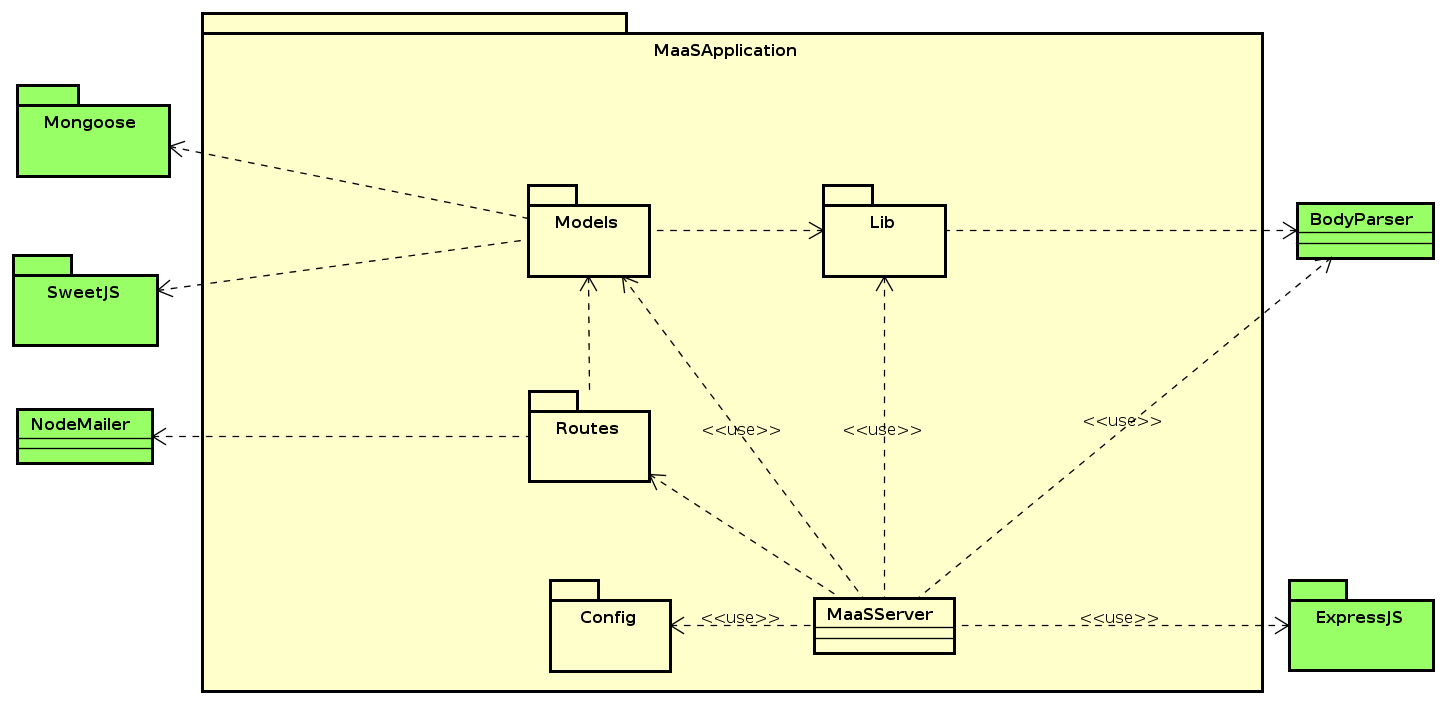
\includegraphics[width=0.8\textwidth]{res/sections/backend/generale.png}
\caption{Diagramma dei \glossaryItem{package}}
\end{figure}

\subsubsection{Package MaaSApplication}
\paragraph*{Descrizione}
Package che racchiude tutta l'applicazione \glossaryItem{MaaS}.

\paragraph*{Package contenuti}
\begin{itemize}
\item Models
\item Routes
\item Config
\item Lib
\end{itemize}

\paragraph*{Classi contenute}
\begin{itemize}
\item MaaSServer
\end{itemize}

\begin{figure}[H]
\centering
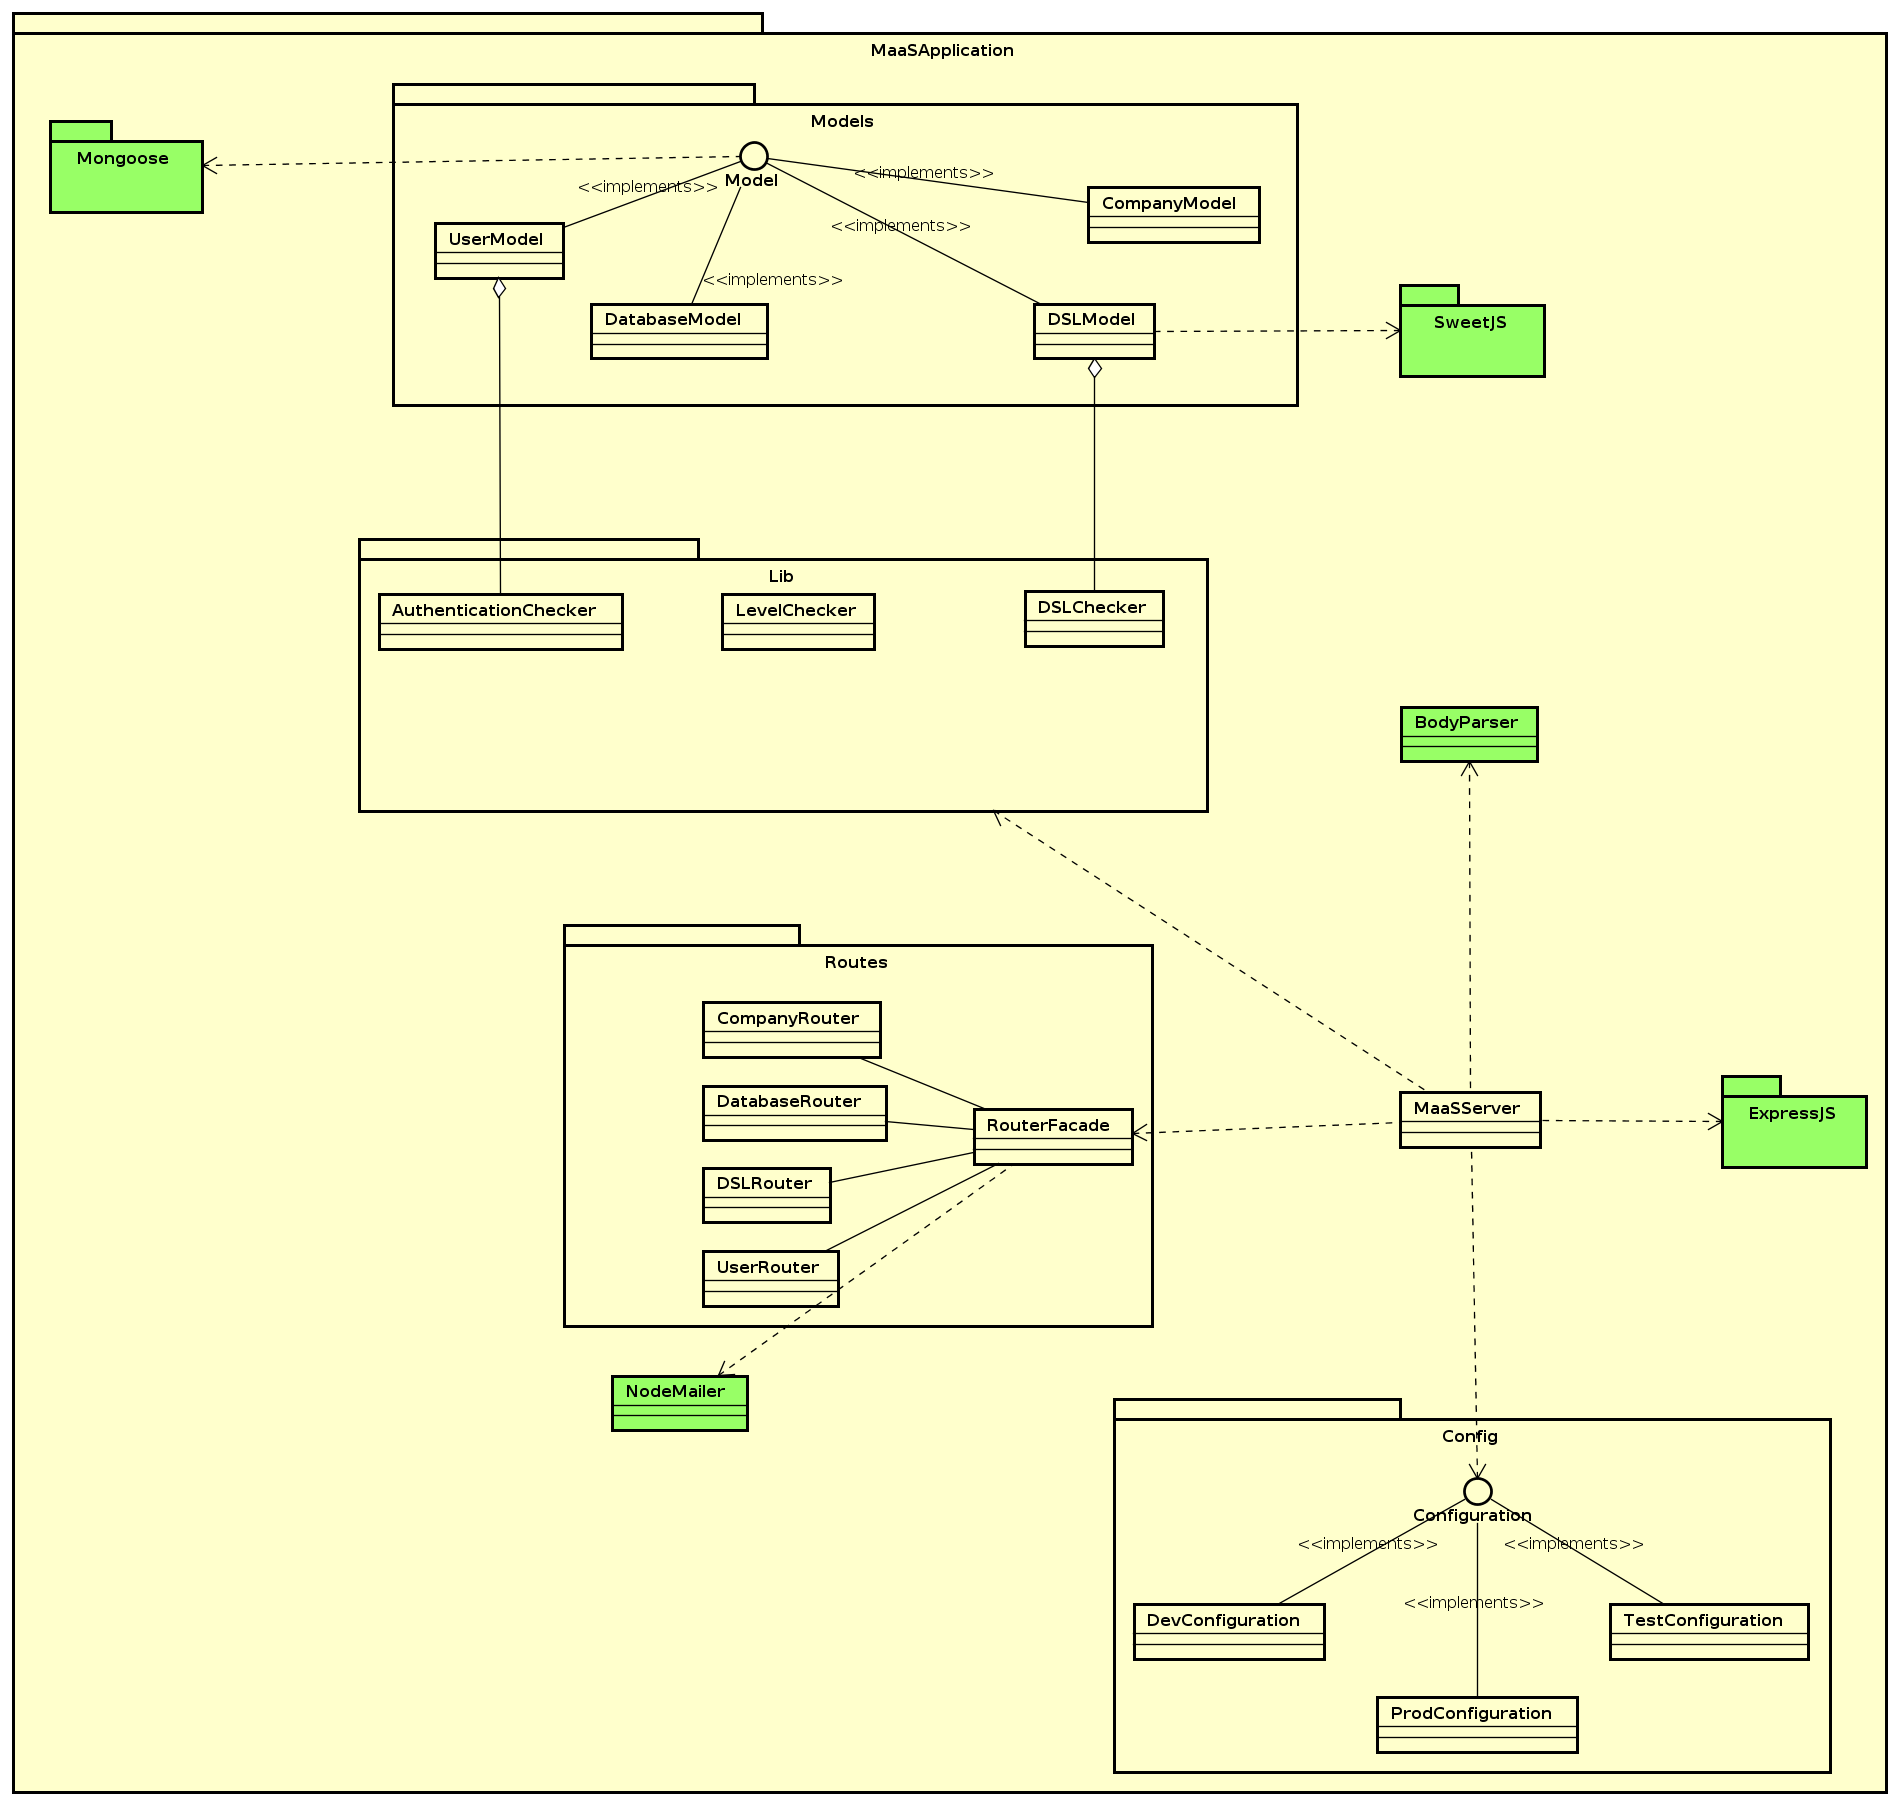
\includegraphics[width=0.8\textwidth]{res/sections/backend/collegamenti.png}
\caption{Diagramma dei \glossaryItem{package} completo dei componenti per ciascun \glossaryItem{package}}
\end{figure}

\subsection{Package Models}
\paragraph*{Descrizione}
Package che racchiude le classi che rappresentano la \textit{business logic} dell'applicazione. Ciascuna di queste classi implementa l'interafaccia Model dichiarata all'interno del \glossaryItem{package}.
Ciascuna classe deve implementare un modello definito da MongooseJS e deve definire i metodi con cui interagire con i dati che la classe stessa rappresenta. \\

\paragraph*{Classi contenute}
\begin{itemize}
\item Model
\item UserModel
\item DSLModel
\item CompanyModel
\item DatabaseModel
\end{itemize}

\begin{figure}[H]
\centering
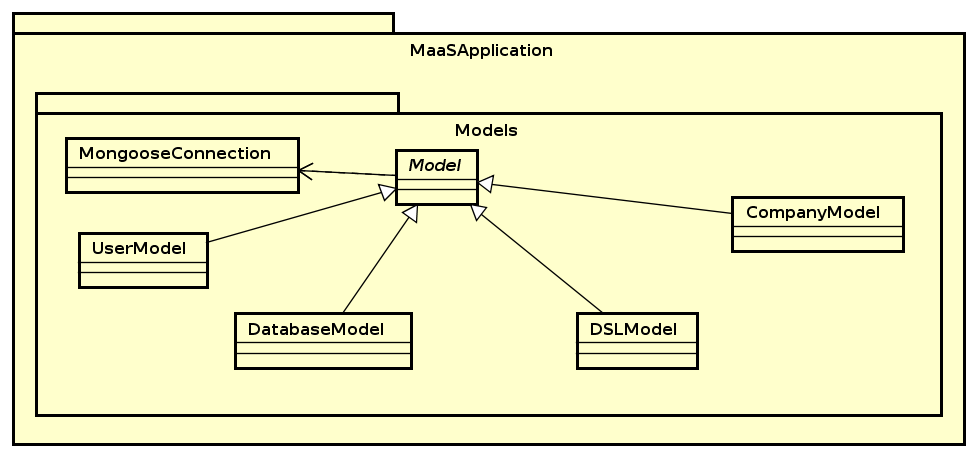
\includegraphics[width=0.8\textwidth]{res/sections/backend/models.png}
\caption{Diagramma delle classi del \glossaryItem{package} Models}
\end{figure}

\paragraph{Model}
\paragraph*{Descrizione}
Classe basa astratta comune a tutti i modelli usati da \glossaryItem{MaaS}.

\paragraph*{Utilizzo}
Viene utilizzata come base per UserModel, CompanyModel, DSLModel e DatabaseModel.

\paragraph*{Relazione con altri \glossaryItem{moduli}}
\begin{itemize}
\item Mongoose, per l'interazione con il database MondoDB dell'applicazione MaaS
\item UserModel, per estensione
\item CompanyModel, per estensione
\item DSLModel, per estensione
\item DatabaseModel, per estensione
\end{itemize}

\subsubsection{UserModel}
\paragraph*{Descrizione}
Classe che racchiude la \textit{business logic} legata agli utenti. Implementa modello e schema definiti da MongooseJS.

\paragraph*{Utilizzo}
Il modello viene utilizzato sia per la rappresentazione di un utente nell'applicazione, sia per l'autenticazione nel sistema.

\paragraph*{Relazioni con altri moduli}
\begin{itemize}
\item Mongoose, per l'interazione con il database MondoDB dell'applicazione MaaS
\item Mongoose-validator, per la validazione degli schemi e dei dati memorizzati
\item Lib::AuthenticationChecker, per il controllo dell'avvenuta autenticazione dell'utente
\item Router::UserRouter, per la gestione delle richieste dirette verso il modello degli utenti
\end{itemize}

\subsubsection{CompanyModel}
\paragraph*{Descrizione}
Racchiude la business logic legata alle \glossaryItem{Company}. Implementa modello e schema definiti da MongooseJS.

\paragraph*{Utilizzo}
Il modello rappresenta una \glossaryItem{Company} nel sistema.

\paragraph*{Relazioni con altri \glossaryItem{moduli}}
\begin{itemize}
\item Mongoose, per l'interazione con il database MondoDB dell'applicazione MaaS
\item Mongoose-validator, per la validazione degli schemi e dei dati memorizzati
\item Router::CompanyRouter, per la gestione delle richieste dirette verso il modello delle Company
\end{itemize}

\paragraph{DatabaseModel}
\paragraph*{Descrizione}

Racchiude la business logic legata al collegamento con i database delle \glossaryItem{Company}. Implementa modello e schema definiti da MongooseJS.

\paragraph*{Utilizzo}
Il modello rappresenta la connessione ad un database aziendale di una \glossaryItem{Company}. Contiene i dati per effettuare l'accesso al database e il riferimento alle collections definite su tale database, permettendo così all'utente di poter definire per ciascuna \glossaryItem{Collection} la possibilità di interagirvi da parte di tutti i membri della propria \glossaryItem{Company} o solo degli Admin.

\paragraph*{Relazioni con altri \glossaryItem{moduli}}
\begin{itemize}
\item Mongoose, per l'interazione con il database MondoDB dell'applicazione MaaS
\item Mongoose-validator, per la validazione degli schemi e dei dati memorizzati
\item Router::DatabaseRouter, per la gestione delle richieste dirette verso il modello dei database
\end{itemize}

\paragraph{DSLModel}
\paragraph*{Descrizione}

Racchiude la \textit{business logic} legata alle specifiche \glossaryItem{DSL}. Implementa modello e schema definiti da MongooseJS.

\paragraph*{Utilizzo}
Il modello viene utilizzato per la rappresentazione delle specifiche \glossaryItem{DSL}. Contiene i dati di tali specifiche e le funzioni per poter estrarre i dati richiesti da una specifica \glossaryItem{DSL}.

\paragraph*{Relazioni con altri \glossaryItem{moduli}}
\begin{itemize}
\item Mongoose, per l'interazione con il database MondoDB dell'applicazione MaaS
\item Mongoose-validator, per la validazione degli schemi e dei dati memorizzati
\item Lib::DSLChecker, per il controllo di validità (sintattica e per la verifica dei permessi di accesso alle Collections di un database) della specifica DSL
\item Router::DSLRouter, per la gestione delle richieste dirette verso il modello delle specifiche DSL
\end{itemize}


\subsubsection{Package Routes}
\paragraph*{Descrizione}
Il \glossaryItem{package} Routes contiene le classi che implementano il router definito da ExpressJS, definendo le varie \glossaryItem{API} esposte dal server.
I \glossaryItem{moduli} vengono suddivisi in base al modello che utilizzano. 
Ciascuna classe inoltre ha il compito di definire i \glossaryItem{middleware} da anteporre alla definizione delle \glossaryItem{API}.\\

\paragraph*{Moduli contenuti}
\begin{itemize}
\item UserRouter
\item CompanyRouter
\item DSLRouter
\item DatabaseRouter
\item RouterFacade
\end{itemize}

\begin{figure}[H]
\centering
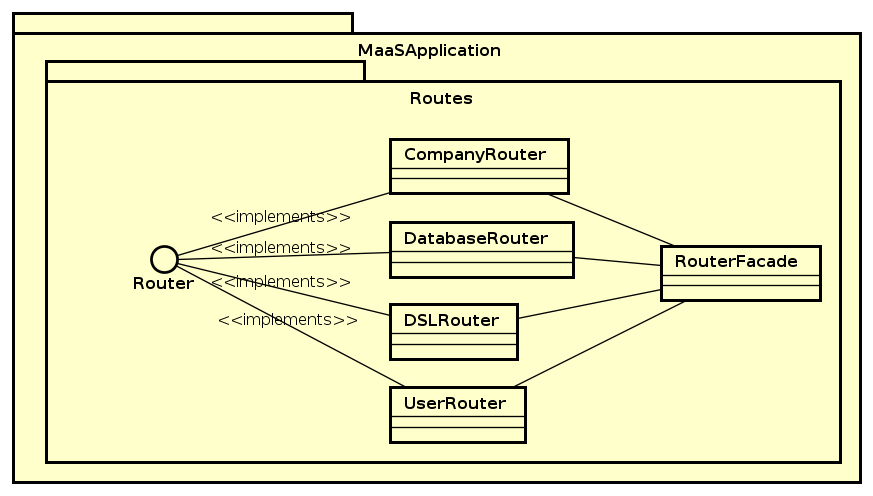
\includegraphics[width=0.8\textwidth]{res/sections/backend/routes.png}
\caption{Diagramma delle classi del \glossaryItem{package} Routes}
\end{figure}

\paragraph{UserRouter}
\paragraph*{Descrizione}
Questa classe contiene la definizione degli endpoint riguardanti gli utenti. 

\paragraph*{Relazione con altri \glossaryItem{moduli}}
\begin{itemize}
\item Lib::AuthenticationChecker
\item Model::UserModel
\end{itemize}

\paragraph{CompanyRouter}
\paragraph*{Descrizione}
Questo \glossaryItem{modulo} contiene la definizione degli endpoint riguardanti le \glossaryItem{Company}.

\paragraph*{Relazione con altri \glossaryItem{moduli}}
\begin{itemize}
\item Lib::AuthenticationChecker, per il controllo dell'avvenuta autenticazione dell'utente
\item Model::CompanyModel, per il soddisfacimento delle richieste verso il modello di dati delle Company
\end{itemize}

\paragraph{DSLRouter}
\paragraph*{Descrizione}
Questo \glossaryItem{modulo} contiene la definizione delle \glossaryItem{API} riguardanti le specifiche \glossaryItem{DSL}.

\paragraph*{Relazione con altri \glossaryItem{moduli}}
\begin{itemize}
\item Lib::AuthenticationChecker, per il controllo dell'avvenuta autenticazione dell'utente
\item Lib::LevelChecker, per il controllo del ruolo dell'utente autenticato
\item Model::DSLModel, per il soddisfacimento delle richieste verso il modello di dati delle specifiche DSL
\end{itemize}

\paragraph{DatabaseRouter}
\paragraph*{Descrizione}
Questo \glossaryItem{modulo} contiene la definizione delle \glossaryItem{API} riguardanti le connessioni ai database aziendali.

\paragraph*{Relazione con altri \glossaryItem{moduli}}
\begin{itemize}
\item Lib::AuthenticationChecker, per il controllo dell'avvenuta autenticazione dell'utente
\item Lib::LevelChecker, per il controllo del ruolo dell'utente autenticato
\item Model::DatabaseModel, per il soddisfacimento delle richieste verso il modello di dati dei database
\end{itemize}

\paragraph{RouterFacade}
\paragraph*{Descrizione}
Oggetto che implementa il Facade \glossaryItem{Design Pattern}. Tale oggetto incorpora tutte le \glossaryItem{API} definite nelle classi Router.

\paragraph*{Relazione con altri \glossaryItem{moduli}}
\begin{itemize}
\item UserRouter
\item CompanyRouter
\item DSLRouter
\item DatabaseRouter
\end{itemize}
Essendo l'implementazione del design pattern Facade, RouterFacade espone un'interfaccia base per il package Routes. I metodi esposti da RouterFacade conterranno chiamate a metodi specifici di UserRouter, CompanyRouter, DSLRouter e DatabaseRouter.

\subsubsection{Package Config}
\paragraph*{Descrizione}
Questo \glossaryItem{package} contiene le classi \glossaryItem{Configuration} che contengono tutte le informazioni per inizializzare correttamente l'applicazione. 
Sarà poi l'applicazione a dover recuperare la corretta configurazione in base alla variabilie d'ambiente NODE\_ENV.

\paragraph*{Moduli contenuti}
\begin{itemize}
\item \glossaryItem{Configuration}
\item DevConfiguration
\item TestConfiguration
\item ProdConfiguration
\end{itemize}

\paragraph*{Interfacce contenute}
\begin{itemize}
\item \glossaryItem{Configuration}
\end{itemize}

\begin{figure}[H]
\centering
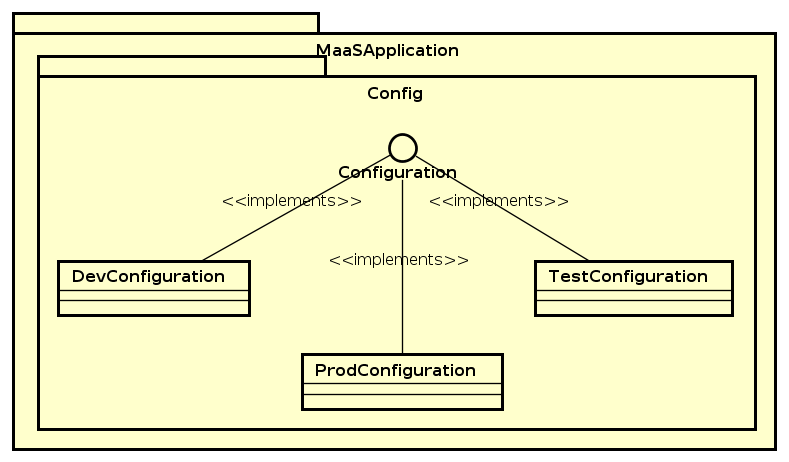
\includegraphics[width=0.8\textwidth]{res/sections/backend/config.png}
\caption{Diagramma delle classi del \glossaryItem{package} Config}
\end{figure}

\paragraph{DevConfiguration}
\paragraph*{Descrizione}
Configurazione usata durante lo sviluppo.

\paragraph*{Utilizzo}
Viene utilizzata per configurare l'ambiente di lavoro durante lo sviluppo di \glossaryItem{MaaS}.

\paragraph{TestConfiguration}
\paragraph*{Descrizione}
Configurazione usata durante il test.

\paragraph*{Utilizzo}
Viene utilizzata per configurare l'ambiente di lavoro durante la \glossaryItem{fase} di test di \glossaryItem{MaaS}.

\paragraph{ProdConfiguration}
\paragraph*{Descrizione}
Configurazione usata per il rilascio.

\paragraph*{Utilizzo}
Viene utilizzata per configurare l'ambiente di lavoro per la consegna di \glossaryItem{MaaS}.

\paragraph{Configuration}
\paragraph*{Descrizione}
Interfaccia comune alle configurazioni usate da \glossaryItem{MaaS}.

\paragraph*{Utilizzo}
Viene utilizzata come base per DevConfiguration, TestConfiguration e ProdConfiguration.

\paragraph*{Relazione con altri \glossaryItem{moduli}}
\begin{itemize}
\item MaaSServer, per la scelta della configurazione dell'applicazione
\end{itemize}

\subsubsection{Package Lib}
\paragraph*{Descrizione}
Questo \glossaryItem{package} contiene tutti i \glossaryItem{moduli} di supporto al sistema e i \glossaryItem{middlewares} generici per ExpressJS.

\paragraph*{Moduli contenuti}
\begin{itemize}
\item LevelChecker
\item AuthenticationChecker
\item DSLChecker
\end{itemize}


\begin{figure}[H]
\centering
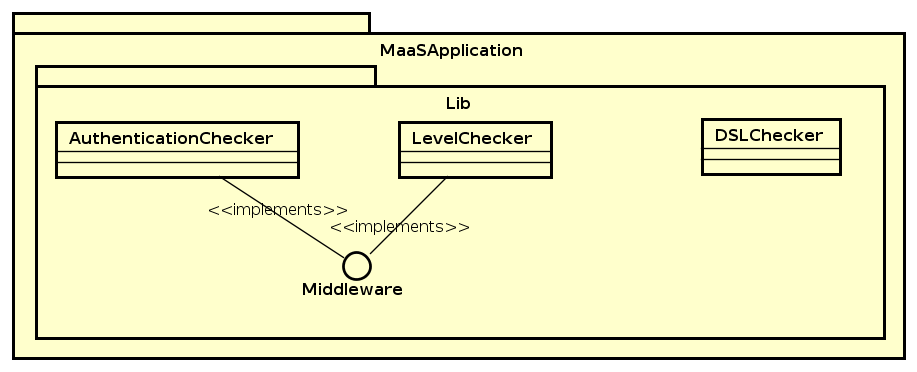
\includegraphics[width=0.8\textwidth]{res/sections/backend/lib.png}
\caption{Diagramma delle classi del \glossaryItem{package} Lib}
\end{figure}

\paragraph{LevelChecker}
\paragraph*{Descrizione}
Middleware che si occupa di verificare se l'utente che effettua una richiesta al server ha i livelli minimi di accesso per poterla eseguire.

\paragraph*{Utilizzo}
Viene utilizzato nelle \textit{routes} in cui deve essere garantito un livello utente minimo di accesso per portare a termine la richiesta.

\paragraph*{Relazione con altri \glossaryItem{moduli}}
\begin{itemize}
\item Router::RouterFacade, per la risposta sul controllo del ruolo dell'utente autenticato
\end{itemize}

\paragraph{AuthenticationChecker}
\paragraph*{Descrizione}
Modulo che definisce due \glossaryItem{middleware}: uno per effettuare il login, l'altro per l'autenticazione di una richiesta.

\paragraph*{Utilizzo}
Questo \glossaryItem{modulo} viene utilizzato per definire l'\textit{endpoint} per effettuare il login all'applicazione e offre il \glossaryItem{middleware} che permette di autenticare le richieste. Tale \glossaryItem{middleware} si occuperà di estrarre il \textit{token} dalle richieste, verificarne la correttezza e aggiungere l'utente verificato nella richiesta per i prossimi \glossaryItem{middleware}.

\paragraph*{Relazione con altri \glossaryItem{moduli}}
\begin{itemize}
\item Router::RouterFacade, per la risposta sul controllo del ruolo dell'utente autenticato
\end{itemize}

\paragraph{DSLChecker}
\paragraph*{Descrizione}
Modulo che \glossaryItem{verifica} la correttezza sintattica e di contenuto di una specifica \glossaryItem{DSL}.

\paragraph*{Utilizzo}
Questo \glossaryItem{modulo} viene richiamato in DSLModel per verificare che la specifica \glossaryItem{DSL} che viene salvata o modificata sia valida per l'esecuzione.

\paragraph*{Relazione con altri \glossaryItem{moduli}}
\begin{itemize}
\item Model::DSLModel, per la risposta sul controllo della validità di una specifica DSL
\end{itemize}

\subsubsection{MaaSServer}
\paragraph*{Descrizione}
Classe principale dell'applicazione.

\paragraph*{Utilizzo}
Viene utilizzata questa classe per inizializzare l'applicazione. Questa classe ha la responsabilità di caricare gli altri \glossaryItem{moduli} del backend correttamente e di inizializzare il webserver che li utilizza.
\paragraph*{Relazione con altri \glossaryItem{moduli}}
\begin{itemize}
\item Config, per la scelta della configurazione dell'applicazione
\item Router::RouterFacade, per la gestione delle API esposte dal server
\item BodyParser, per il parsing del corpo della richiesta
\item ExpressJS, per la creazione ed esposizione delle API REST
\end{itemize}

\subsection{API REST}
\subsubsection{Comunicazione tra client e server}
Per la creazione del backend di \glossaryItem{MaaS} si è deciso di utilizzare \glossaryItem{Node.js} e, in particolare, il \glossaryItem{framework} ExpressJS, che permette la creazione semplificata di server \glossaryItem{REST}. Il lato backend sarà quindi costituito da un insieme di \glossaryItem{API} protette da strati diversi di sicurezza. \\
Ciascuna \glossaryItem{API} del webserver fornirà una risposta in formato \glossaryItem{JSON} per permettere la fruizione delle informazioni. Fornirà nello stesso formato anche gli eventuali messaggi di errore generati nel corpo dei metodi del server. Tali messaggi di errore saranno così composti: 
\begin{verbatim}
{
    "code":     [Codice definito nel protocollo HTTP, che identifica univocamente
                 la tipologia del problema]
    "message":  [Messaggio che definisce in dettaglio la tipologia dell'errore]
    ["data":   [Opzionale, trasporta i dati in cui si è verificato l'errore]]
}
\end{verbatim}
I codici di errore saranno del tipo 4xx (client error, la richiesta è sintatticamente scorretta o non può essere soddisfatta) o 5xx (server error, il server ha fallito nel soddisfare una richiesta apparentemente valida).
\subsubsection{Sicurezza}
Gli accessi alle \glossaryItem{API} avranno 2 livelli di sicurezza. \\
Il primo livello è rappresentato dall'autenticazione: un utente non autenticato riceverà un errore se richiede una \glossaryItem{API} protetta. Verrà implementato con l'utilizzo di PassportJS, un \glossaryItem{middleware} per ExpressJS che permette l'autenticazione di utenti nel sistema. In particolare verrà utilizzata la strategia passport-local per l'accesso al server, cioè le credenziali dell'utente risiederanno nel database locale. \\
Il secondo livello è definito in base al ruolo di appartenenza di un utente. Si occuperà di controllare i permessi assegnati ad un utente autenticato e di verificare la possibilità che possa o meno interagire con la risorsa richiesta. \\
I ruoli utente ammessi nell'applicazione sono: 
\begin{itemize}
\item \textbf{Guest};
\item \textbf{Member};
\item \textbf{Admin};
\item \textbf{Owner};
\item \textbf{Super Admin}.
\end{itemize}
Per il ruolo di Super Admin è abilititato un set di \glossaryItem{API} per la gestione dell'intera applicazione. Tali \glossaryItem{API} non sono accessibili agli utenti con altri ruoli.
\newpage
\subsubsection{Scenari di accesso negato}
Di seguito verranno rappresentati \glossaryItem{scenari} corrispondenti ad una negazione di accesso per ruolo non conforme alle attese o per errore nel login.
\paragraph{Errore di autenticazione}  \mbox{} \\
\textbf{Descrizione:} L'utente non autenticato cerca di accedere a \glossaryItem{MaaS}, ma la \glossaryItem{procedura} di login rileva un errore nelle credenziali inserite.
\begin{figure}[H]
\centering
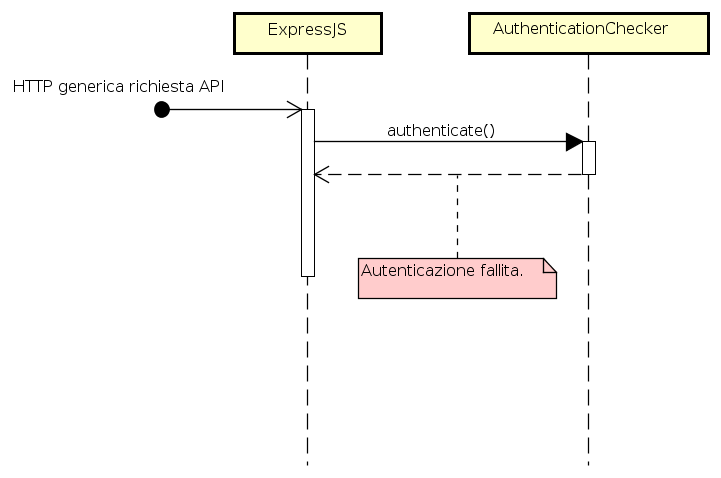
\includegraphics[width=0.8\textwidth]{res/sections/backend/sequence/autenticazioneFallita.png}
\caption{Autenticazione fallita}
\end{figure}
\paragraph{Livello minimo: MEMBER} \mbox{} \\
\textbf{Descrizione:} Tentativo di accesso ad una risorsa visibile solo a utenti con ruolo almeno MEMBER da parte di un utente GUEST.
\begin{figure}[H]
\centering
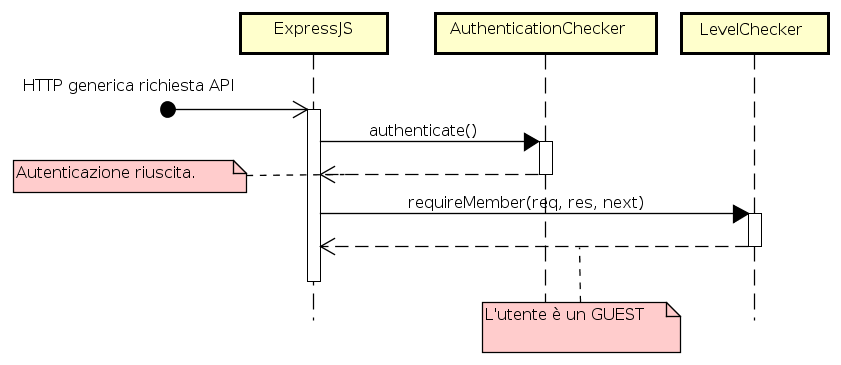
\includegraphics[width=0.8\textwidth]{res/sections/backend/sequence/requireMemberFallita.png}
\caption{Livello minimo MEMBER}
\end{figure}
\paragraph{Livello minimo: ADMIN} \mbox{} \\
\textbf{Descrizione:} Tentativo di accesso ad una risorsa visibile solo a utenti con ruolo almeno ADMIN da parte di un utente GUEST o MEMBER.
\begin{figure}[H]
\centering
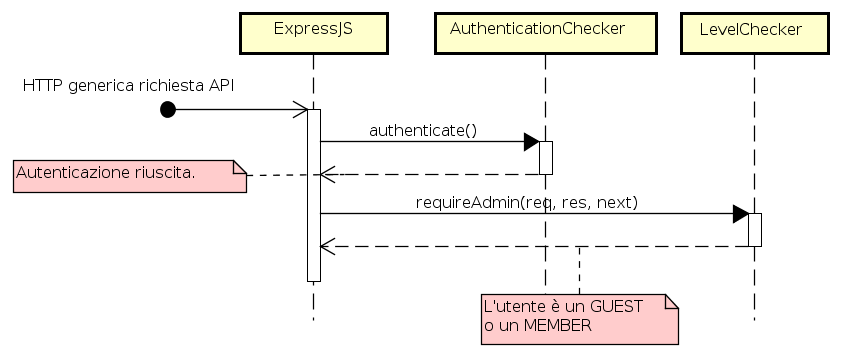
\includegraphics[width=0.8\textwidth]{res/sections/backend/sequence/requireAdminFallita.png}
\caption{Livello minimo ADMIN}
\end{figure}
\paragraph{Livello minimo: OWNER}  \mbox{} \\
\textbf{Descrizione:} Tentativo di accesso ad una risorsa visibile solo a utenti con ruolo almeno OWNER da parte di un utente GUEST, MEMBER o ADMIN.
\begin{figure}[H]
\centering
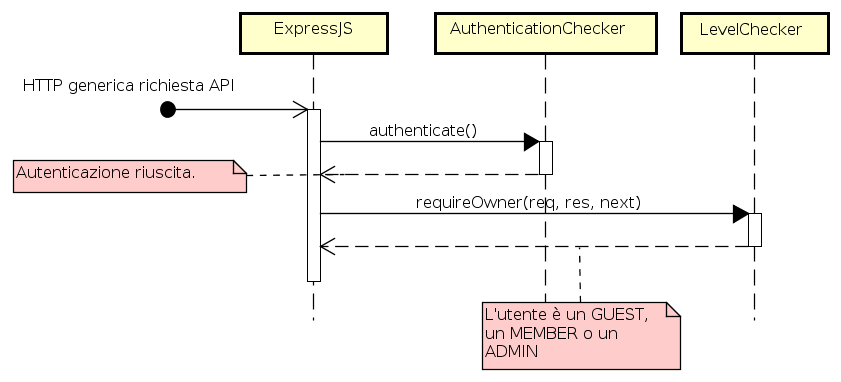
\includegraphics[width=0.8\textwidth]{res/sections/backend/sequence/requireOwnerFallita.png}
\caption{Livello minimo OWNER}
\end{figure}
\paragraph{Livello minimo: SUPERADMIN}  \mbox{} \\
\textbf{Descrizione:} Tentativo di accesso ad una risorsa accedibile solo da un SUPERADMIN da parte di un generico utente di \glossaryItem{MaaS}.
\begin{figure}[H]
\centering
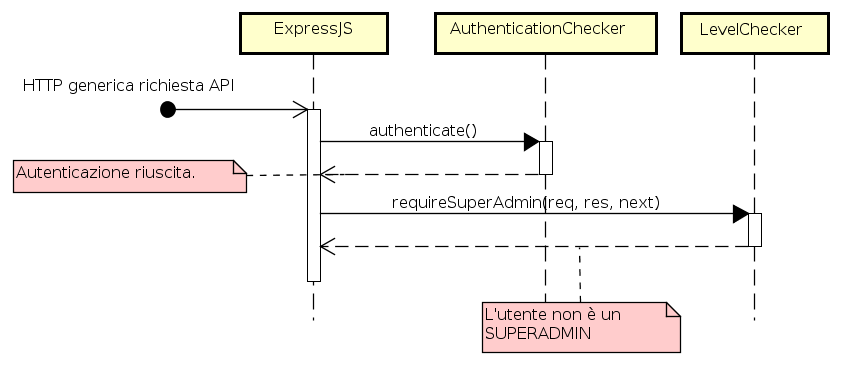
\includegraphics[width=0.8\textwidth]{res/sections/backend/sequence/requireSuperAdminFallita.png}
\caption{Livello minimo SUPERADMIN}
\end{figure}
\newpage
\subsection{Descrizione API}
Di seguito sono descritte le \glossaryItem{API} \glossaryItem{REST} esposte dal server di \glossaryItem{MaaS}. Si suppone che l'utente che richiede l'accesso alla risorsa descritta abbia i permessi necessari (ovvero che sia autenticato e che il suo ruolo sia conforme a quanto indicato). Qualora questo non fosse vero si ricadrebbe in uno degli \glossaryItem{scenari} esposti precedentemente.
\subsubsection{Senza autenticazione}
\paragraph{Login}\mbox{}\\
\textbf{Tipologia:} POST \\
\textbf{API:} /api/login \\
\textbf{Descrizione:} Necessita di una richiesta con \textit{body} contenente email e password dell'utente. Lo scopo della richiesta è quello di autenticare l'utente presso MaaS e di rendergli disponibili funzionalità dipendenti dal suo ruolo e dai suoi permessi. \\
\textbf{Scenario:} 
\begin{figure}[H]
\centering
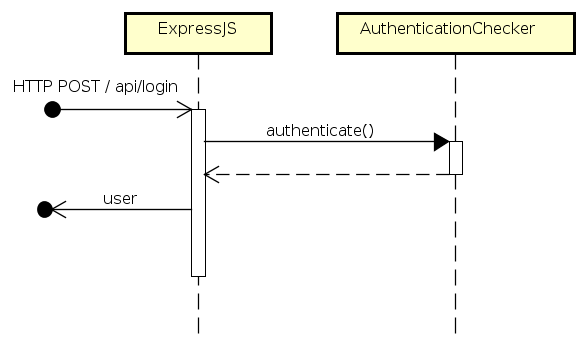
\includegraphics[width=0.8\textwidth]{res/sections/backend/sequence/(POST)login.png}
\caption{Scenario del login}
\end{figure}

\newpage
\paragraph{Registrazione}\mbox{}\\
\textbf{Tipologia:} POST \\
\textbf{API:} /api/register/:unique\_code \\
\textbf{Descrizione:} Metodo per la creazione di un utente invitato da una \glossaryItem{Company}. Necessita di una richiesta con \textit{body} contenete le informazioni per la creazione completa di un utente, in particolare indirizzo email, password e Company di riferimento. A seguito della richiesta un nuovo utente è registrato presso MaaS e collegato alla Company. \\
\textbf{Scenario:} 
\begin{figure}[H]
\centering
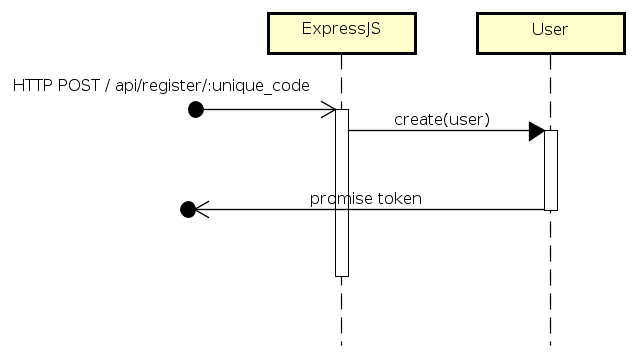
\includegraphics[width=0.8\textwidth]{res/sections/backend/sequence/(POST)register.png}
\caption{Scenario della registrazione}
\end{figure}

\newpage
\paragraph{Creazione Company}\mbox{}\\
\textbf{Tipologia:} POST \\
\textbf{API:} /api/companies \\
\textbf{Descrizione:} Necessita di una richiesta con \textit{body} contenente le informazioni relative alla \glossaryItem{Company} e alla creazione del profilo del suo \glossaryItem{Owner}. Queste informazioni includono indirizzo email e password dell'Owner e nome della Company da creare. \\
\textbf{Scenario:} 
\begin{figure}[H]
\centering
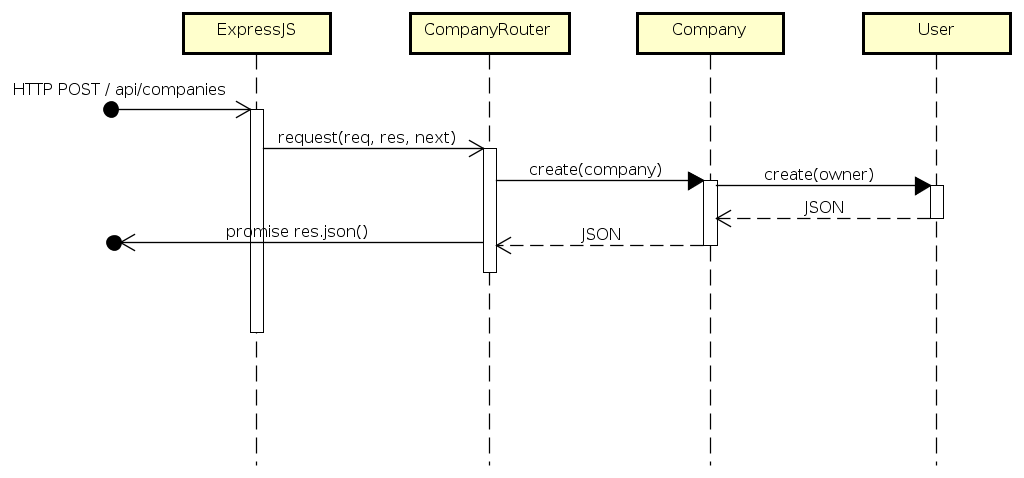
\includegraphics[width=0.8\textwidth]{res/sections/backend/sequence/(POST)company.png}
\caption{Scenario della creazione \glossaryItem{company}}
\end{figure}

\newpage
\subsubsection{User}

\paragraph{Inserimento utente}\mbox{}\\
\textbf{Tipologia:} POST \\
\textbf{API:} /api/companies/:company\_id/users \\
\textbf{Livello di accesso minimo:} OWNER \\
\textbf{Descrizione:} Necessita di una richiesta con \textit{body} contenente l'email e il livello di accesso dell'utente da creare, che viene memorizzato presso il database interno di MaaS; i permessi di cui godrà sono dipendenti dal ruolo scelto, e possono essere modificati in qualsiasi momento da un Admin o da un Owner. Per accertare che sia l'Owner ad inviare la richiesta viene controllato il livello dell'utente autenticato. \\
\textbf{Scenario:} 
\begin{figure}[H]
\centering
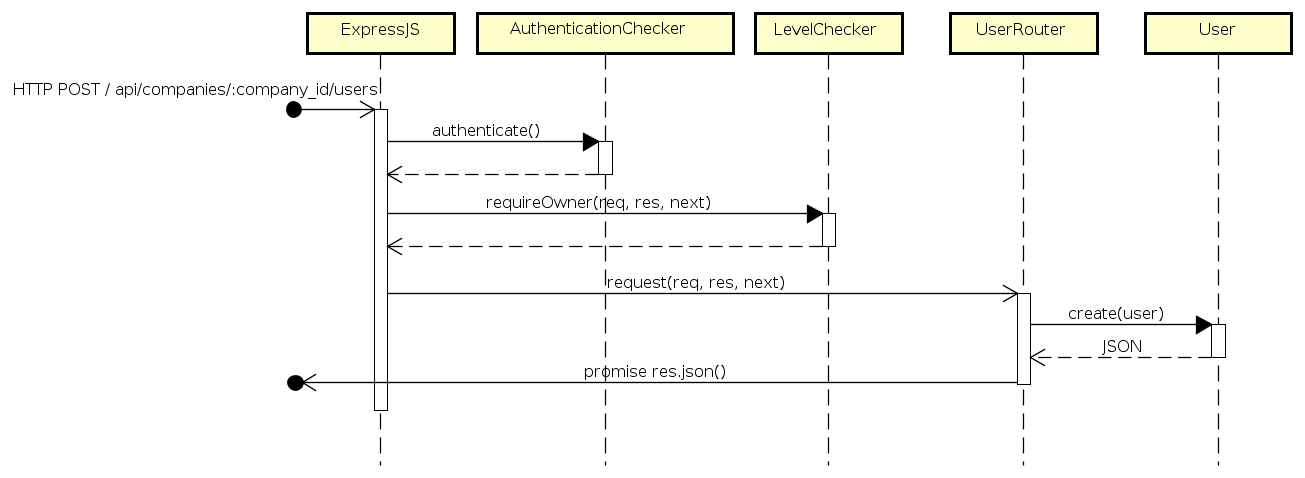
\includegraphics[width=0.8\textwidth]{res/sections/backend/sequence/(POST)user.png}
\caption{Scenario dell'inserimento utente in una \glossaryItem{Company}}
\end{figure}

\newpage
\paragraph{Aggiornamento delle credenziali utente}\mbox{}\\
\textbf{Tipologia:} PUT \\
\textbf{API:} /api/companies/:company\_id/users/:user\_id/credentials \\
\textbf{Livello di accesso minimo:} GUEST \\
\textbf{Descrizione:} Necessita di una richiesta con \textit{body} contenente le nuove credenziali di accesso dell'utente, in particolare indirizzo email e nuova password. Ovviamente un utente ha il permesso di cambiare solo le proprie credenziali, ed essendo l'indirizzo email unico prima dell'aggiornamento viene fatto un controllo per assicurare il rispetto di questo vincolo. Nel caso in cui l'indirizzo emailsia già esistente, viene restituito un errore. \\
\textbf{Scenario:} 
\begin{figure}[H]
\centering
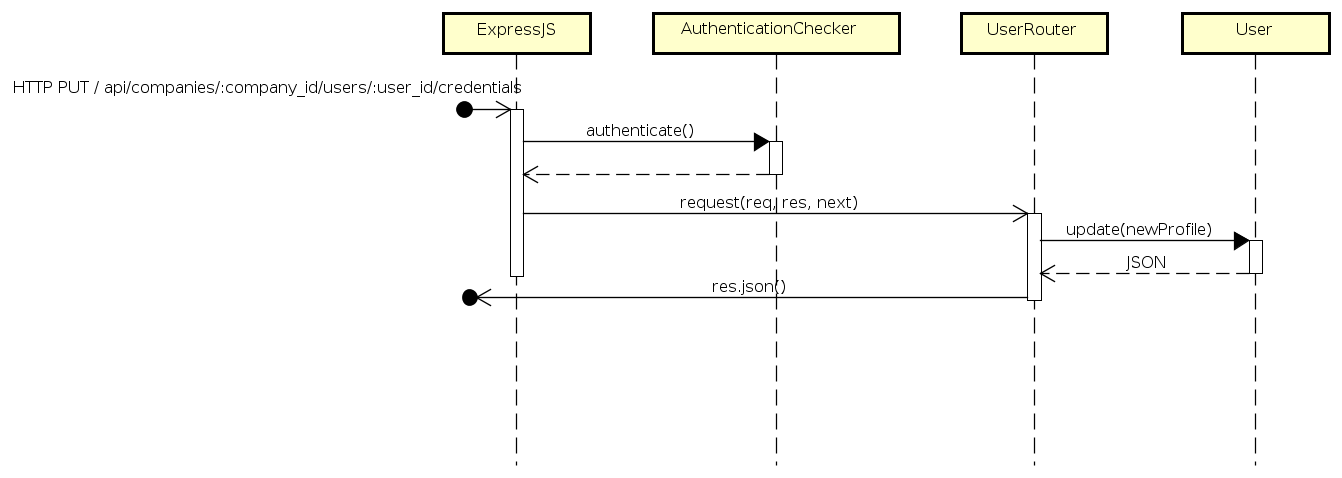
\includegraphics[width=0.8\textwidth]{res/sections/backend/sequence/(PUT)credenzialiUtente.png}
\caption{Scenario dell'aggiornamento delle credenziali di un utente}
\end{figure}

\newpage
\paragraph{Cancellazione utente}\mbox{}\\
\textbf{Tipologia:} DELETE \\
\textbf{API:} /api/companies/:company\_id/users/:user\_id \\
\textbf{Livello di accesso minimo:} OWNER \\
\textbf{Descrizione:} L'utente della Company con ID :company\_id corrispondente all'utente con ID :user\_id viene rimosso dal database di MaaS e scollegato dalla Company di appartenza. A seguito della richiesta viene ritornato messaggio di conferma dell'avvenuta cancellazione. \\
\textbf{Scenario:} 
\begin{figure}[H]
\centering
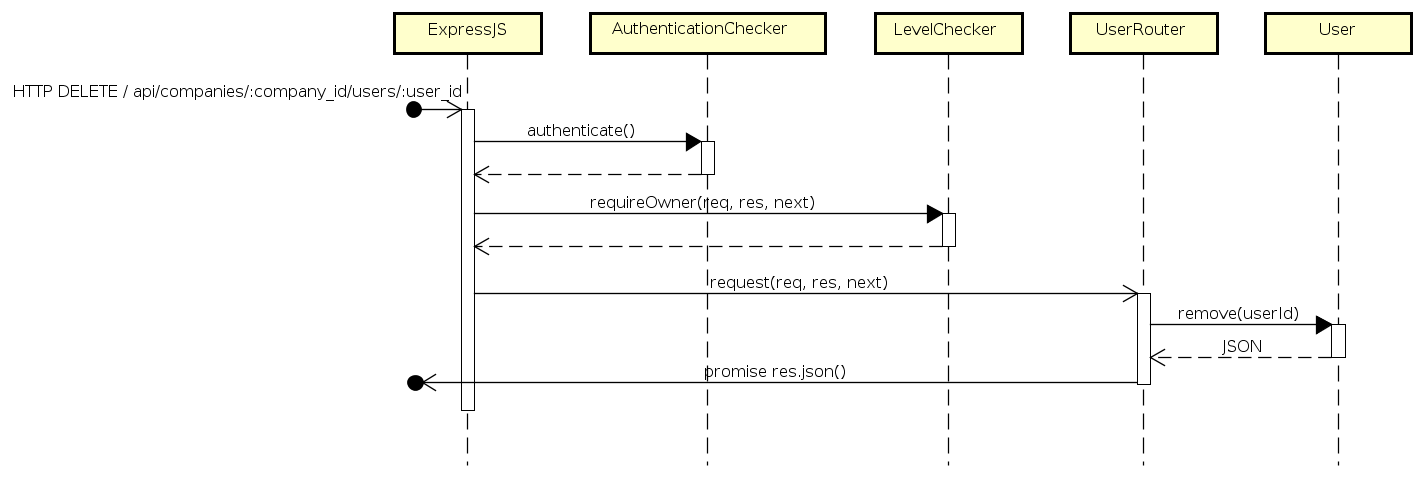
\includegraphics[width=0.8\textwidth]{res/sections/backend/sequence/(DELETE)user.png}
\caption{Scenario della cancellazione utente da una \glossaryItem{company}}
\end{figure}

\newpage
\subsubsection{Company}
\paragraph{Dati di una Company}\mbox{}\\
\textbf{Tipologia:} GET \\
\textbf{API:} /api/companies/:company\_id/ \\
\textbf{Livello di accesso minimo:} GUEST \\
\textbf{Descrizione:} Ritorna le informazioni generali della \glossaryItem{Company} corrispondente all'ID :company\_id. Se la Company non esiste viene ritornato un messagio di errore, altrimenti vengono ritornati il nome della Company e l'indirizzo email del suo Owner. \\
\textbf{Scenario:} 
\begin{figure}[H]
\centering
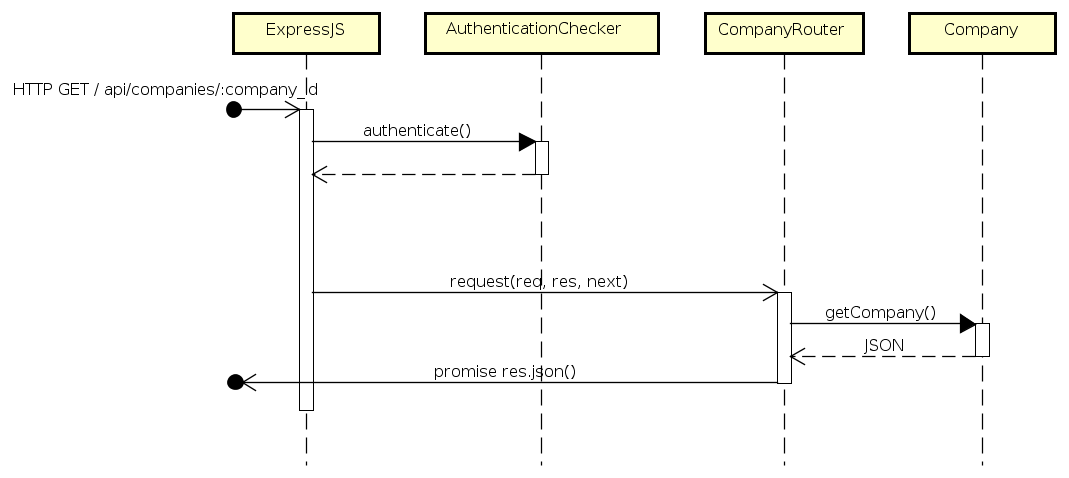
\includegraphics[width=0.8\textwidth]{res/sections/backend/sequence/(GET)company.png}
\caption{Scenario di ottenimento dei dati di una \glossaryItem{Company}}
\end{figure}

\newpage
\paragraph{Aggiornamento dei dati di una Company}\mbox{}\\
\textbf{Tipologia:} PUT \\
\textbf{API:} /api/companies/:company\_id/ \\
\textbf{Livello di accesso minimo:} ADMIN \\
\textbf{Descrizione:} Necessita di una richiesta con \textit{body} contenente le modifiche da apportare ai dati della \glossaryItem{Company} corrispondente all'ID :company\_id. Se la Company non esiste viene ritornato un messagio di errore. \\
\textbf{Scenario:} 
\begin{figure}[H]
\centering
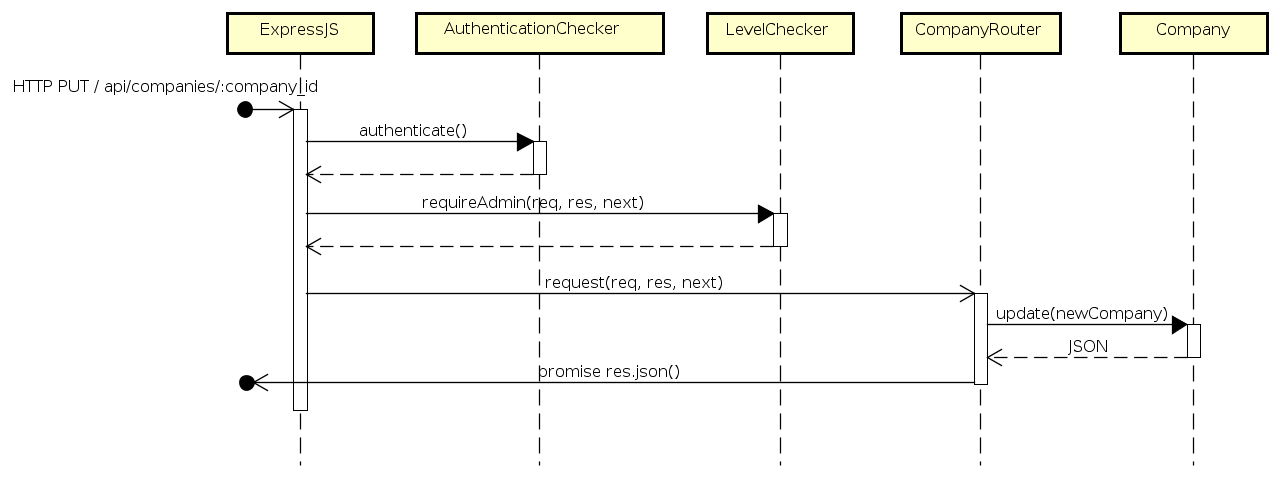
\includegraphics[width=0.8\textwidth]{res/sections/backend/sequence/(PUT)company.png}
\caption{Scenario dell'aggiornamento dei dati di una \glossaryItem{Company}}
\end{figure}

\newpage
\paragraph{Cancellazione di una Company}\mbox{}\\
\textbf{Tipologia:} DELETE \\
\textbf{API:} /api/companies/:company\_id/ \\
\textbf{Livello di accesso minimo:} OWNER \\
\textbf{Descrizione:} Rimuove la Company corrispondente all'ID :company\_id. Se la Company non esiste viene ritornato un messagio di errore, altrimenti viene restituita una conferma di cancellazione. La cancellazione della Company comporta anche la cancellazione di tutti gli utenti associati ad essa. \\
\textbf{Scenario:} 
\begin{figure}[H]
\centering
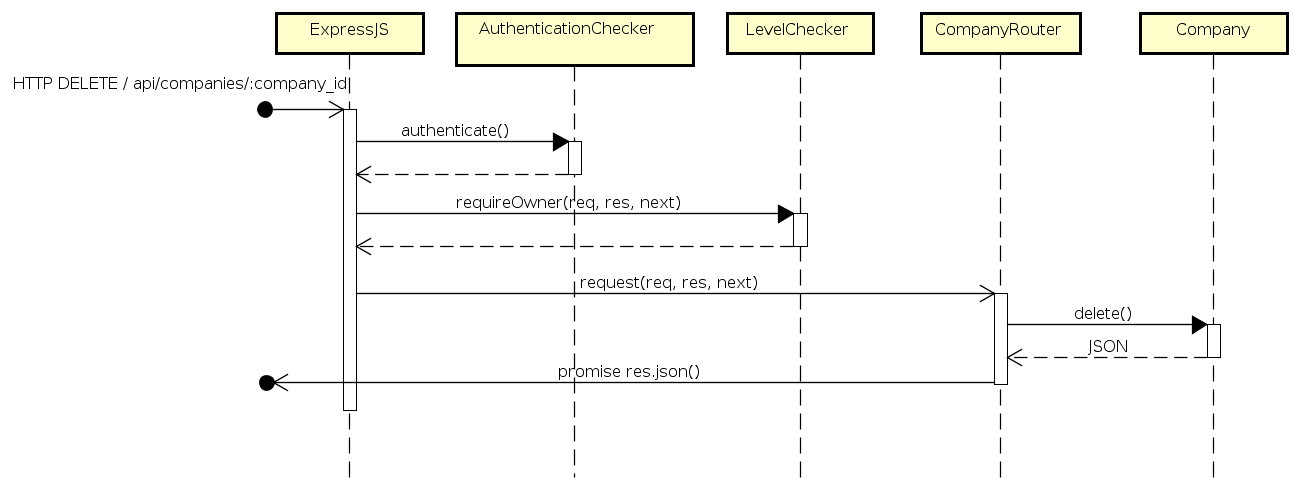
\includegraphics[width=0.8\textwidth]{res/sections/backend/sequence/(DELETE)company.png}
\caption{Scenario della cancellazione di una \glossaryItem{Company}}
\end{figure}

\newpage
\subsubsection{DSL}
\paragraph{Elenco delle specifiche DSL}\mbox{}\\
\textbf{Tipologia:} GET \\
\textbf{API:} /api/companies/:company\_id/DSLs \\
\textbf{Livello di accesso minimo:} GUEST \\
\textbf{Descrizione:} Ritorna un array contenente le specifiche \glossaryItem{DSL} alle quali l'utente ha accesso in formato \glossaryItem{JSON}. Questo array potrebbe essere vuoto, nel caso in cui l'utente non avesse accesso a nessuna specifica DSL; in caso contrario contiene ogni informazione necessaria a distinguere le specifiche l'una dall'altra. A partire da questo elenco l'utente, dipendentemente da ruoli e permessi, può eseguire, leggere o modificare una specifica DSL. \\
\textbf{Scenario:} 
\begin{figure}[H]
\centering
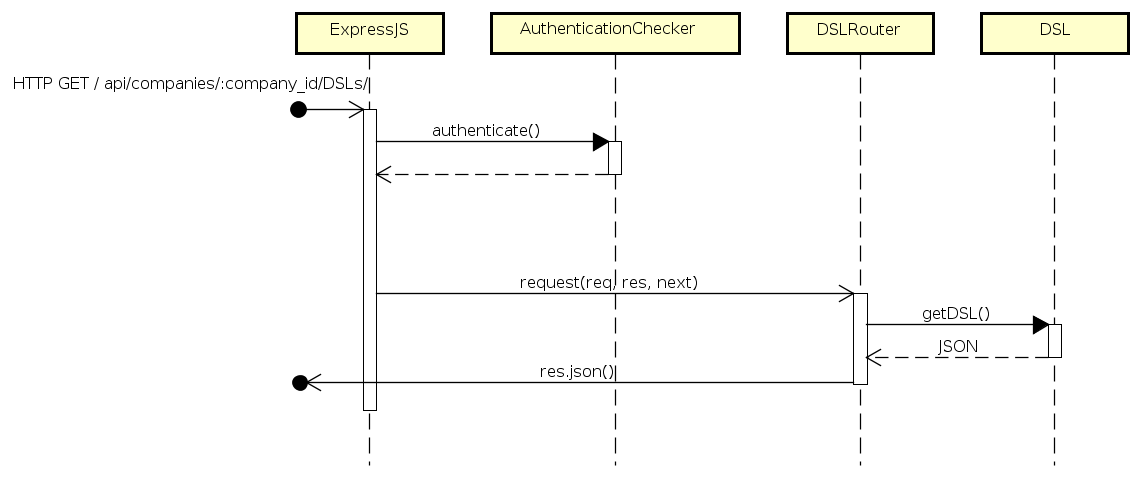
\includegraphics[width=0.8\textwidth]{res/sections/backend/sequence/(GET)dsl.png}
\caption{Scenario dell'elenco delle specifiche \glossaryItem{DSL}}
\end{figure}

\newpage
\paragraph{Lettura del codice di una specifica DSL}\mbox{}\\
\textbf{Tipologia:} GET \\
\textbf{API:} /api/companies/:company\_id/DSLs/:dsl\_id \\
\textbf{Livello di accesso minimo:} MEMBER \\
\textbf{Descrizione:} Ritorna il codice della specifica \glossaryItem{DSL} richiesta in formato \glossaryItem{JSON}. \\
\textbf{Scenario:} 
\begin{figure}[H]
\centering
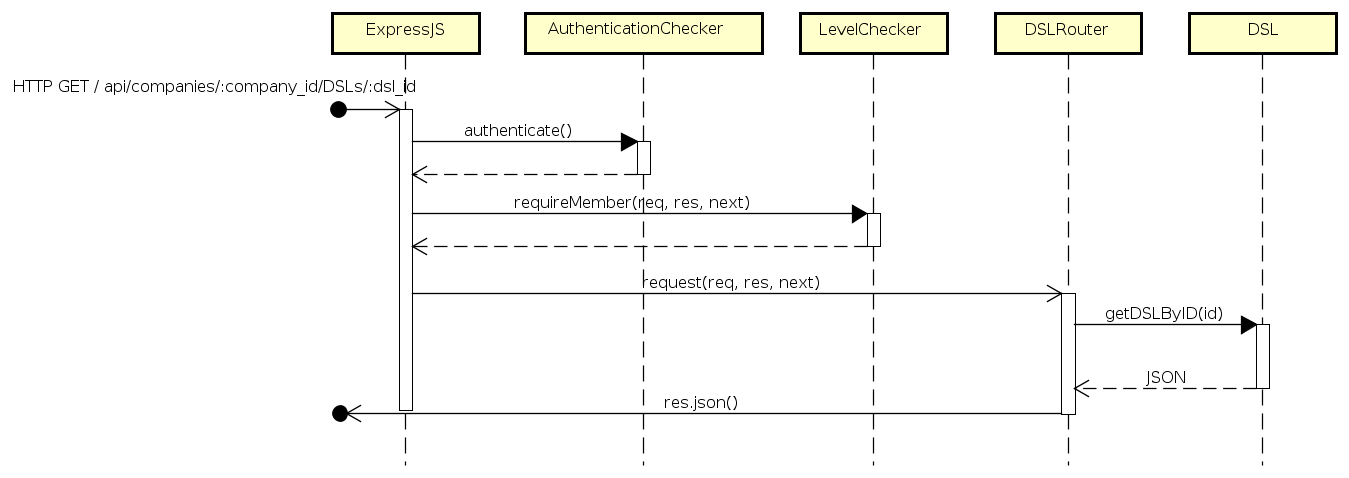
\includegraphics[width=0.8\textwidth]{res/sections/backend/sequence/(GET)dslByID.png}
\caption{Scenario della lettura del codice di una specifica \glossaryItem{DSL}}
\end{figure}

\newpage
\paragraph{Aggiunta di una specifica DSL}\mbox{}\\
\textbf{Tipologia:} POST \\
\textbf{API:} /api/companies/:company\_id/DSLs \\
\textbf{Livello di accesso minimo:} MEMBER \\
\textbf{Descrizione:} Necessita di una richiesta con \textit{body} contenente i dati necessari alla creazione della specifica \glossaryItem{DSL}. La specifica DSL viene validata, in modo da assicurare che non acceda a Collection non accedibili dagli utenti Member e che sia sintatticamente corretta. Se questi controlli vengono superati con successo la specifica DSL viene salvata e associata alla Company, con la restituzione di un messaggio di conferma, altrimenti viene ritornato un messagio di errore. \\
\textbf{Scenario:} 
\begin{figure}[H]
\centering
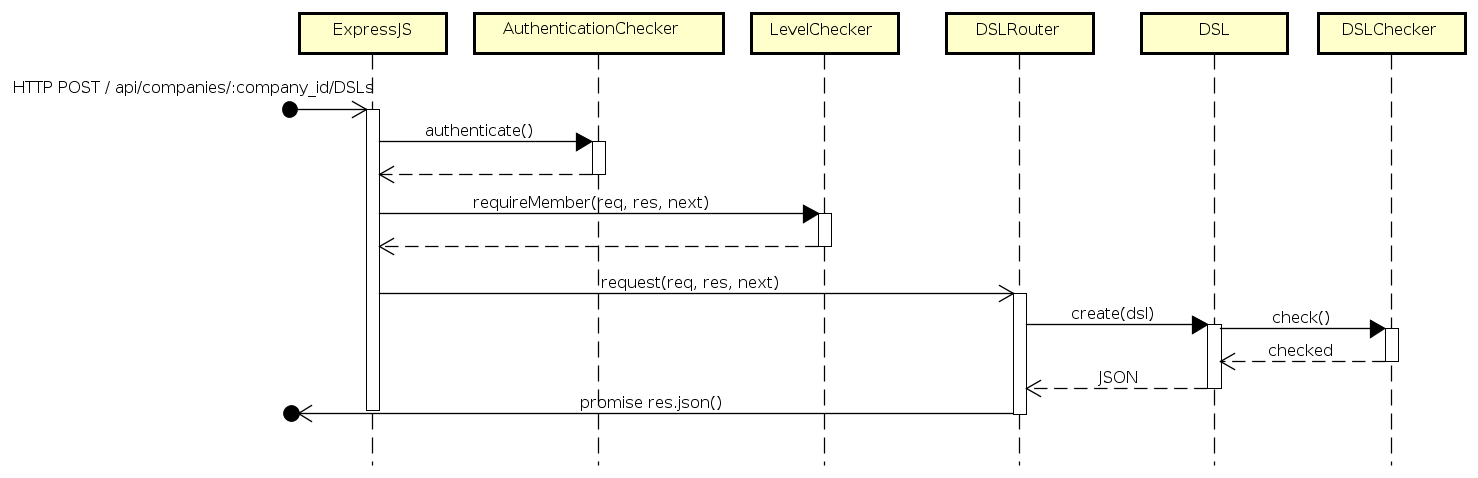
\includegraphics[width=0.8\textwidth]{res/sections/backend/sequence/(POST)dsl.png}
\caption{Scenario della creazione di una specifica \glossaryItem{DSL}}
\end{figure}

\newpage
\paragraph{Aggiornamento del codice di una specifica DSL}\mbox{}\\
\textbf{Tipologia:} PUT \\
\textbf{API:} /api/companies/:company\_id/DSLs/:dsl\_id \\
\textbf{Livello di accesso minimo:} MEMBER \\
\textbf{Descrizione:} Necessita di una richiesta con body contenente i dati necessari alla modifica della specifica \glossaryItem{DSL} identificata da dsl\_id. Tutti i controlli descritti per la creazione della specifica DSL vengono ripetuti, in modo da assicurare che la modifica non abbia introdotto errori. Anche in questo caso, se i controlli vengono superati con successo la specifica DSL viene salvata, con la restituzione di un messaggio di conferma, altrimenti viene ritornato un messagio di errore. \\
\textbf{Scenario:}
\begin{figure}[H]
\centering
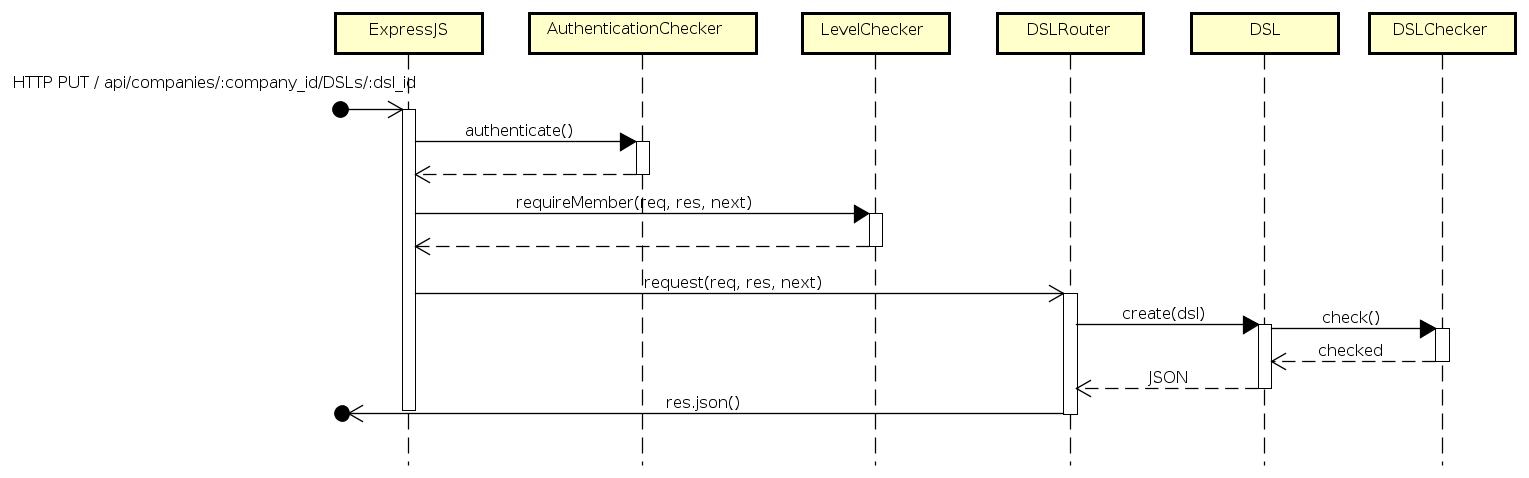
\includegraphics[width=0.8\textwidth]{res/sections/backend/sequence/(PUT)dsl.png}
\caption{Scenario dell'aggiornamento del codice di una specifica \glossaryItem{DSL}}
\end{figure}

\newpage
\paragraph{Cancellazione di una specifica DSL}\mbox{}\\
\textbf{Tipologia:} DELETE \\
\textbf{API:} /api/companies/:company\_id/DSLs/:dsl\_id \\
\textbf{Livello di accesso minimo:} MEMBER \\
\textbf{Descrizione:} Ritorna un messaggio in formato \glossaryItem{JSON} di avvenuta cancellazione se esiste una specifica DSL corrispondente a :dsl\_id, altrimenti viene ritornato un messaggio di errore. \\
\textbf{Scenario:} 
\begin{figure}[H]
\centering
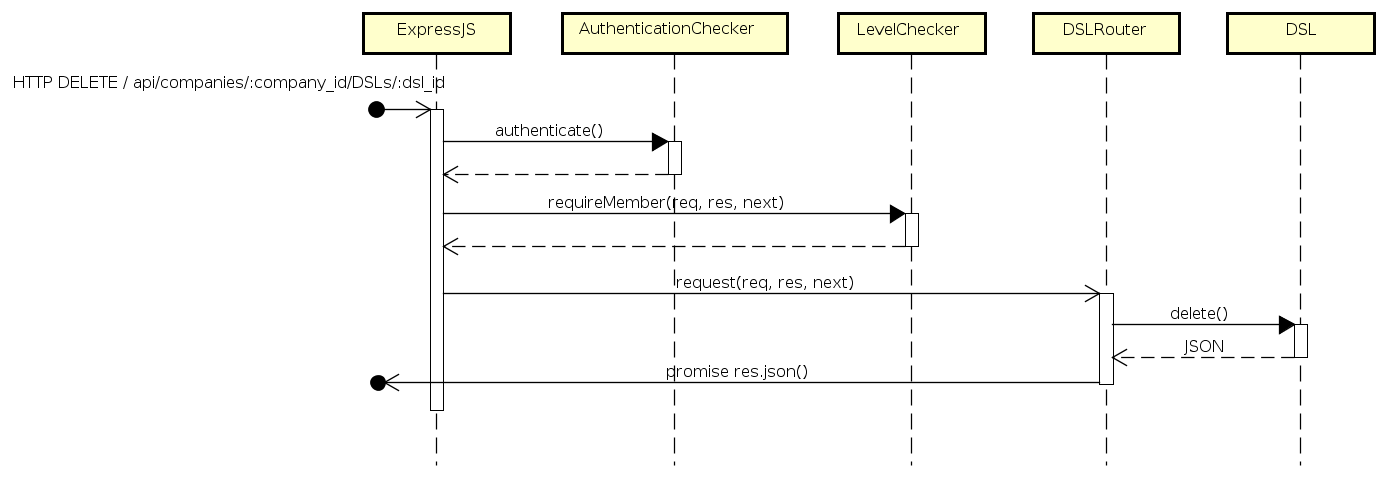
\includegraphics[width=0.8\textwidth]{res/sections/backend/sequence/(DELETE)dsl.png}
\caption{Scenario della cancellazione di una specifica \glossaryItem{DSL}}
\end{figure}

\newpage
\paragraph{Ottenimento della Dashboard di un utente}\mbox{}\\
\textbf{Tipologia:} GET \\
\textbf{API:} /api/companies/:company\_id/users/:user\_id/dashboard \\
\textbf{Livello di accesso minimo:} GUEST \\
\textbf{Descrizione:} Ritorna la \glossaryItem{Dashboard} di un utente definita da una specifica \glossaryItem{DSL}. Ovviamente potrebbe non esistere una specifica DSL che descrive la Dashboard di un utente: in questo caso viene restituita la Dashboard di default contente le specifiche DSL accedibili dall'utente. \\
\textbf{Scenario:}  
\begin{figure}[H]
\centering
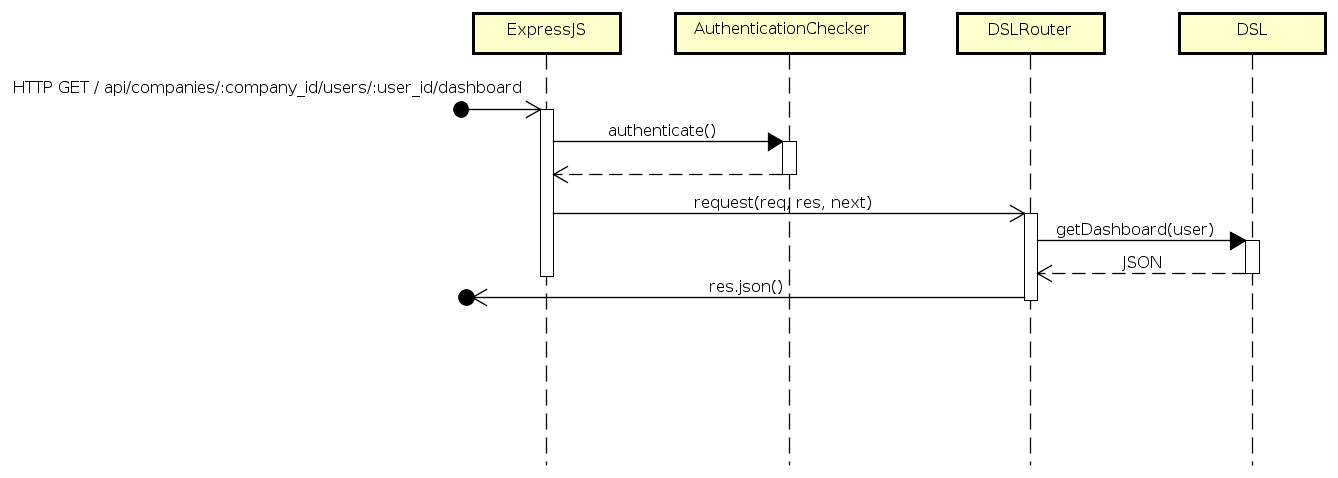
\includegraphics[width=0.8\textwidth]{res/sections/backend/sequence/(GET)dashboard.png}
\caption{Scenario dell'ottenimento della \glossaryItem{Dashboard} di un utente}
\end{figure}

\newpage
\paragraph{Esecuzione di una specifica DSL}\mbox{}\\
\textbf{Tipologia:} GET \\
\textbf{API:} /api/companies/:company\_id/DSLs/:dsl\_id/execute \\
\textbf{Livello di accesso minimo:} GUEST \\
\textbf{Descrizione:} Ritorna un \glossaryItem{JSON} contenente i dati richiesti dalla specifica \glossaryItem{DSL} e la struttura su cui inserire i dati. In questo modo eventuali funzioni inserite nella specifica DSL possono essere esguite lato client, evitando di bloccare l'esecuzione lato server nel caso di funzioni maligne inserite per un tentativo di attacco di tipo DoS (\textbf{D}enial \textbf{o}f \textbf{S}ervice. \\
\textbf{Scenario:} 
\begin{figure}[H]
\centering
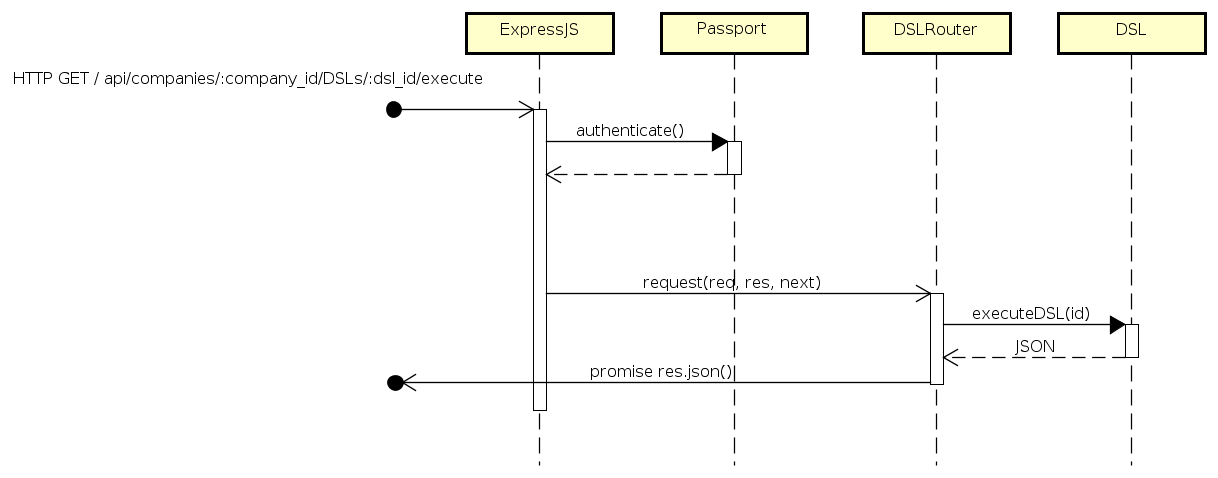
\includegraphics[width=0.8\textwidth]{res/sections/backend/sequence/(GET)dslByIDex.png}
\caption{Scenario dell'esecuzione di una specifica \glossaryItem{DSL}}
\end{figure}

\newpage
\subsubsection{Database}
\paragraph{Elenco dei database della Company}\mbox{}\\
\textbf{Tipologia:} GET \\
\textbf{API:} /api/companies/:company\_id/databases \\
\textbf{Livello di accesso minimo:} MEMBER \\
\textbf{Descrizione:} Ritorna un array contenente i nomi e gli id di ciascun database. In questo modo un utente sa come riferirsi ad un database nella scrittura di una specifica DSL. \\
\textbf{Scenario:}
\begin{figure}[H]
\centering
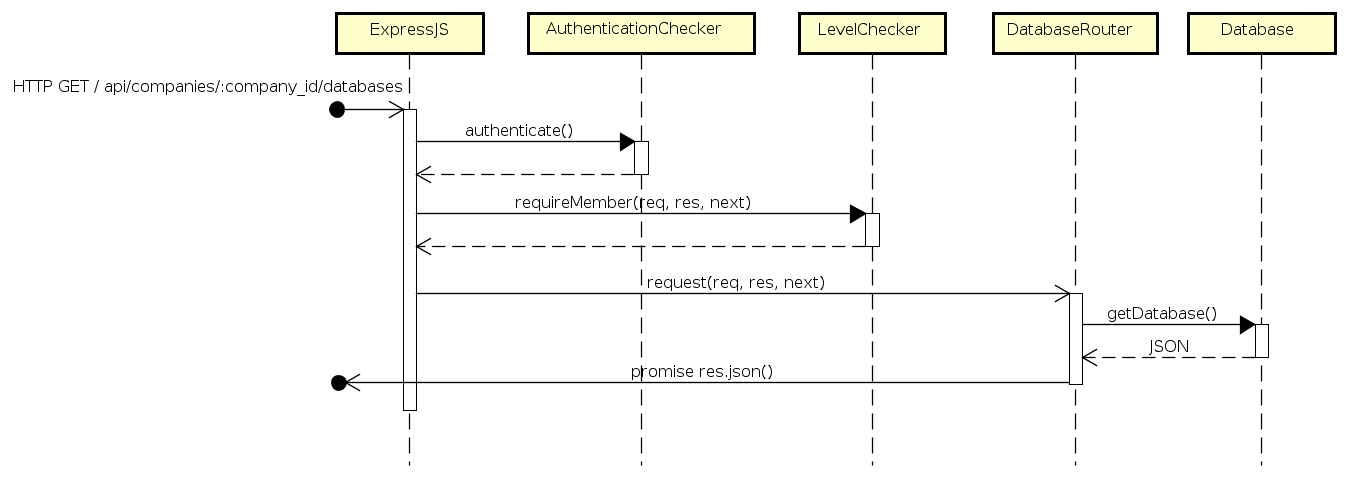
\includegraphics[width=0.8\textwidth]{res/sections/backend/sequence/(GET)database.png}
\caption{Scenario dell'elenco dei database propri della \glossaryItem{Company}}
\end{figure}

\newpage
\paragraph{Visualizzazione dati di un database}\mbox{}\\
\textbf{Tipologia:} GET \\
\textbf{API:} /api/companies/:company\_id/databases/:database\_id \\
\textbf{Livello di accesso minimo:} ADMIN \\
\textbf{Descrizione:} Ritorna tutte le informazioni relative al database richiesto: le credenziali dell'utente appositamente creato per la lettura dei dati, il nome del database, l'host e la porta. Queste informazioni compongono la stringa di connessione necessaria per accedere al database. \\
\textbf{Scenario:} 
\begin{figure}[H]
\centering
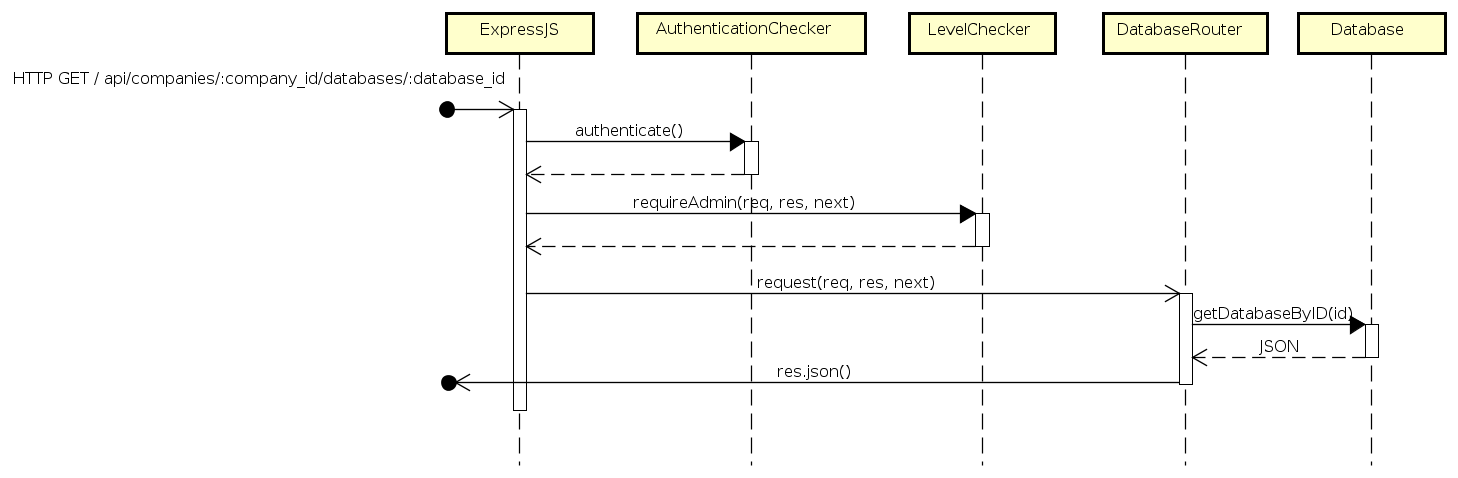
\includegraphics[width=0.8\textwidth]{res/sections/backend/sequence/(GET)databaseById.png}
\caption{Scenario della visualizzazione dei dati di un database}
\end{figure}

\newpage
\paragraph{Aggiunta di un database}\mbox{}\\ 
\textbf{Tipologia:} POST \\
\textbf{API:} /api/companies/:company\_id/databases \\
\textbf{Livello di accesso minimo:} ADMIN \\
\textbf{Descrizione:} Necessita di una richiesta con \textit{body} contenete i dati relativi alla connessione del nuovo database, in particolare le credenziali dell'utente appositamente creato per la lettura dei dati, il nome del database, l'host e la porta. A seguito della richiesta viene ritornato un messaggio di conferma o di errore, dipendentemente dall'esito. \\
\textbf{Scenario:}
\begin{figure}[H]
\centering
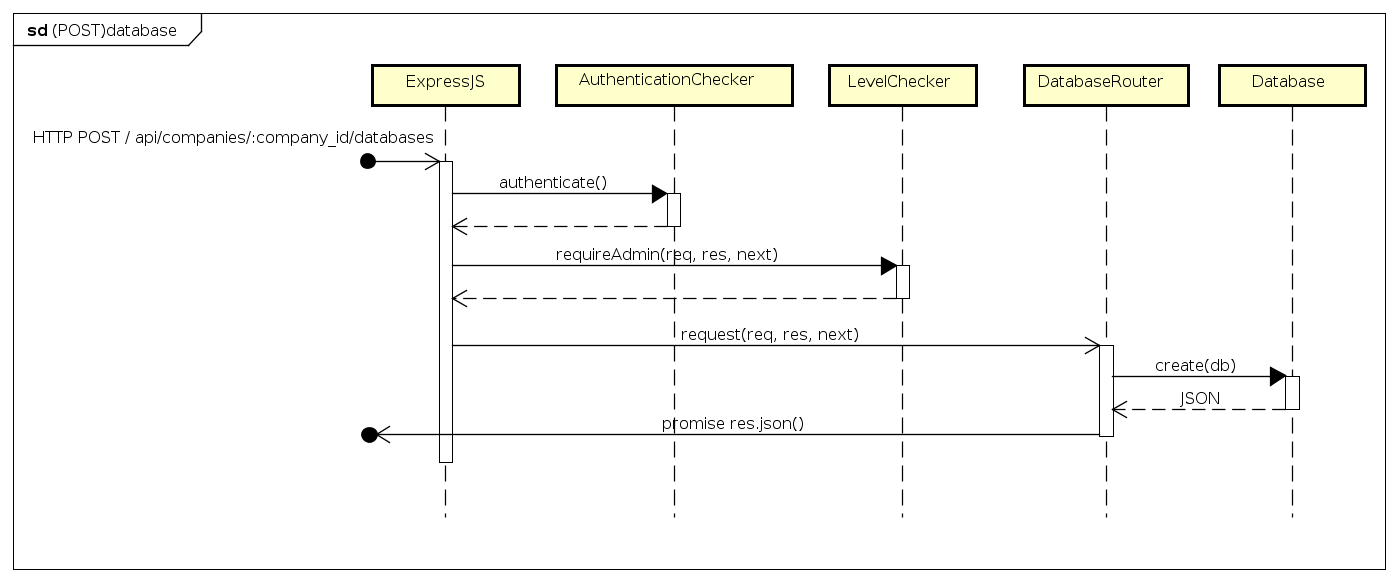
\includegraphics[width=0.8\textwidth]{res/sections/backend/sequence/(POST)database.png}
\caption{Scenario di aggiunta di un database}
\end{figure}

\newpage
\paragraph{Aggiornamento di un database}\mbox{}\\
\textbf{Tipologia:} PUT \\
\textbf{API:} /api/companies/:company\_id/databases/:database\_id \\
\textbf{Livello di accesso minimo:} ADMIN \\
\textbf{Descrizione:} Necessita di una richiesta con \textit{body} contenete i dati relativi alla connessione del database da modificare, in particolare le credenziali dell'utente appositamente creato per la lettura dei dati, il nome del database, l'host e la porta. A seguito della richiesta viene ritornato un messaggio di conferma o di errore, dipendentemente dall'esito. A differenza del procedimento di creazione, tuttavia, la richiesta di modifica viene usata anche per aggiungere, o rimuovere, le Collections del database. Le informazioni richieste per una Collection sono il nome e la conferma di accessibilità da parte di utenti Member. \\
\textbf{Scenario:}
\begin{figure}[H]
\centering
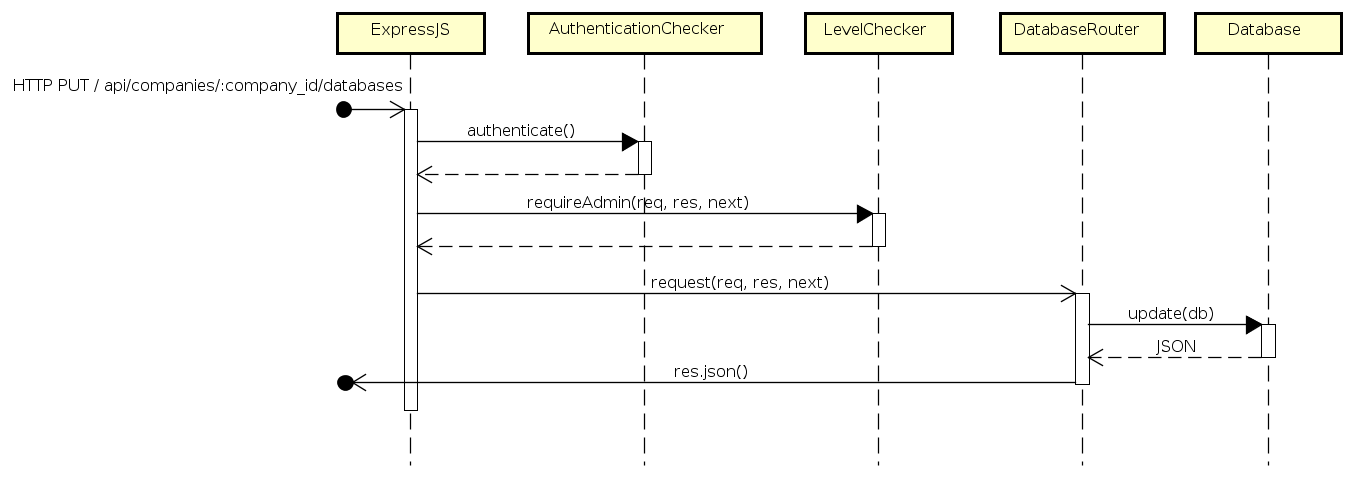
\includegraphics[width=0.8\textwidth]{res/sections/backend/sequence/(PUT)database.png}
\caption{Scenario dell'aggiornamento di un database}
\end{figure}

\newpage
\paragraph{Cancellazione di un database}\mbox{}\\
\textbf{Tipologia:} DELETE \\
\textbf{API:} /api/companies/:company\_id/databases/:database\_id \\
\textbf{Livello di accesso minimo:} ADMIN \\
\textbf{Descrizione:} Elimina il database selezionato, tutte le specifiche \glossaryItem{DSL} che lo utilizzano e le Collections ad esso collegate. Lesecuzione di questa richiesta comporta un pericoloso effetto domino che può portare a distruggere i dati di una Company. \\
\textbf{Scenario:} 
\begin{figure}[H]
\centering
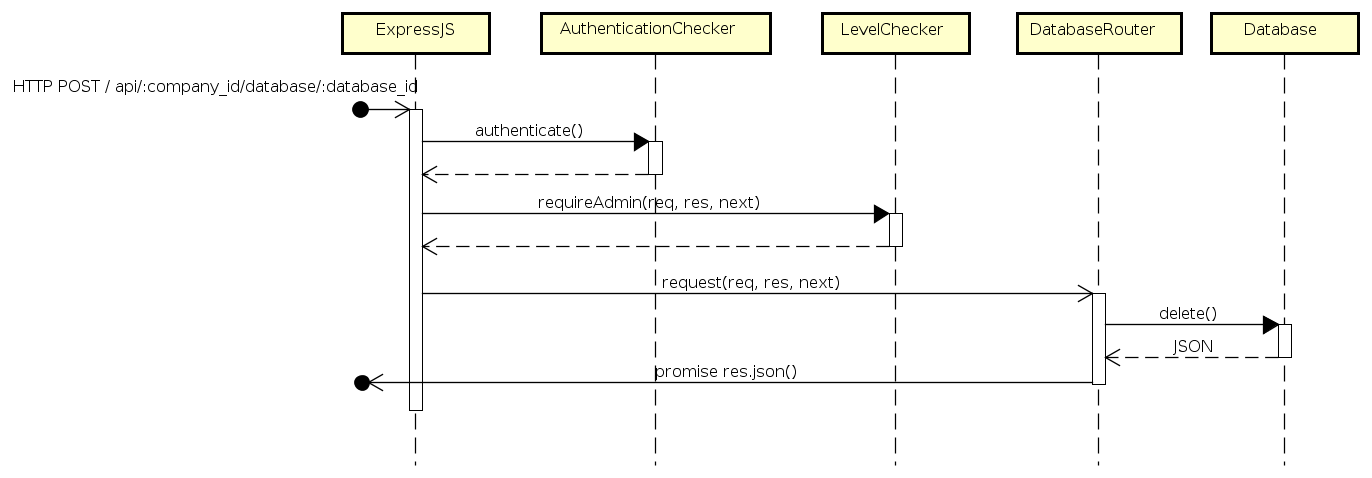
\includegraphics[width=0.8\textwidth]{res/sections/backend/sequence/(DELETE)database.png}
\caption{Scenario della cancellazione di un database}
\end{figure}

\newpage
\paragraph{Visualizzazione Collections di un database} \mbox{}\\
\textbf{Tipologia:} GET \\
\textbf{API:} /api/companies/:company\_id/databases/:database\_id/collections \\
\textbf{Livello di accesso minimo:} MEMBER \\
\textbf{Descrizione:} Ritorna un array di \glossaryItem{Collection} relative ad un database a cui l'utente ha accesso. L'array ritornato può essere vuoto: questo accade quando l'utente non ha accesso a nessuna Collection di quel database. \\
\textbf{Scenario:} 
\begin{figure}[H]
\centering
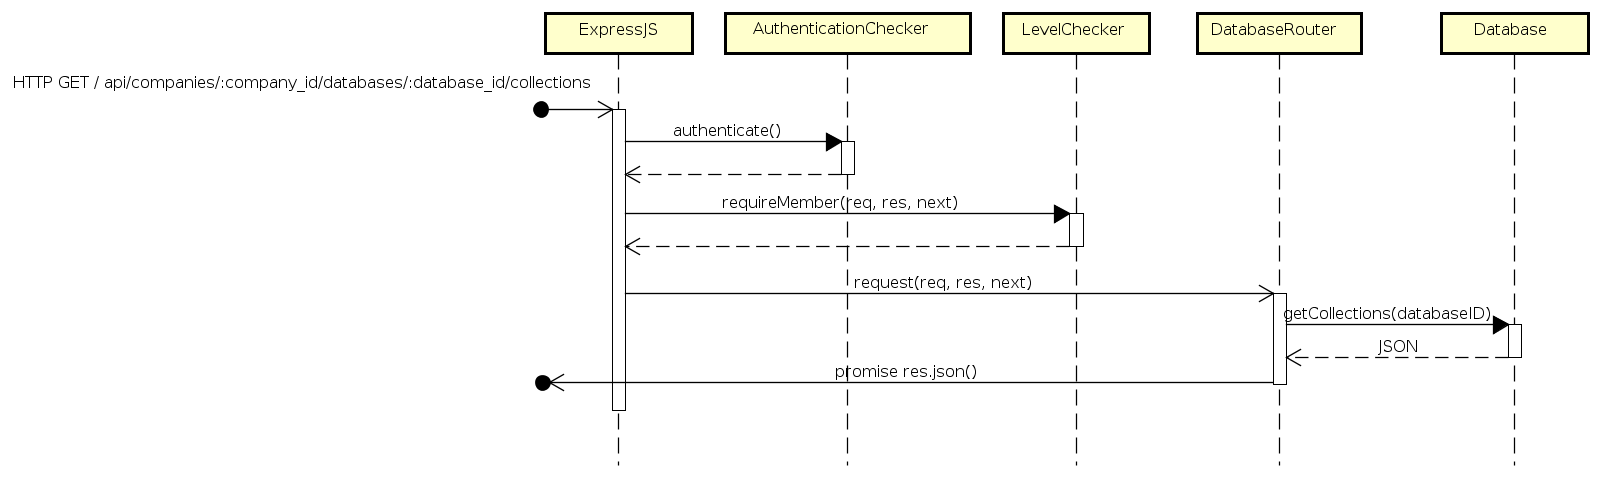
\includegraphics[width=0.8\textwidth]{res/sections/backend/sequence/(GET)collection.png}
\caption{Scenario della visualizzazione Collections di un database}
\end{figure}

\newpage
\subsubsection{Super admin}
\paragraph{Ottenimento informazioni delle Company}\mbox{}\\
\textbf{Tipologia:} GET \\
\textbf{API:} /api/admin/companies \\
\textbf{Descrizione:} Restituisce un array di \glossaryItem{JSON} contenenti le informazioni relative alle \glossaryItem{Company} presenti nell'applicazione, in particolare nome e indirizzo email dell'Owner. Se non sono presenti Company l'array ritornato è vuoto. \\
\textbf{Scenario:} 
\begin{figure}[H]
\centering
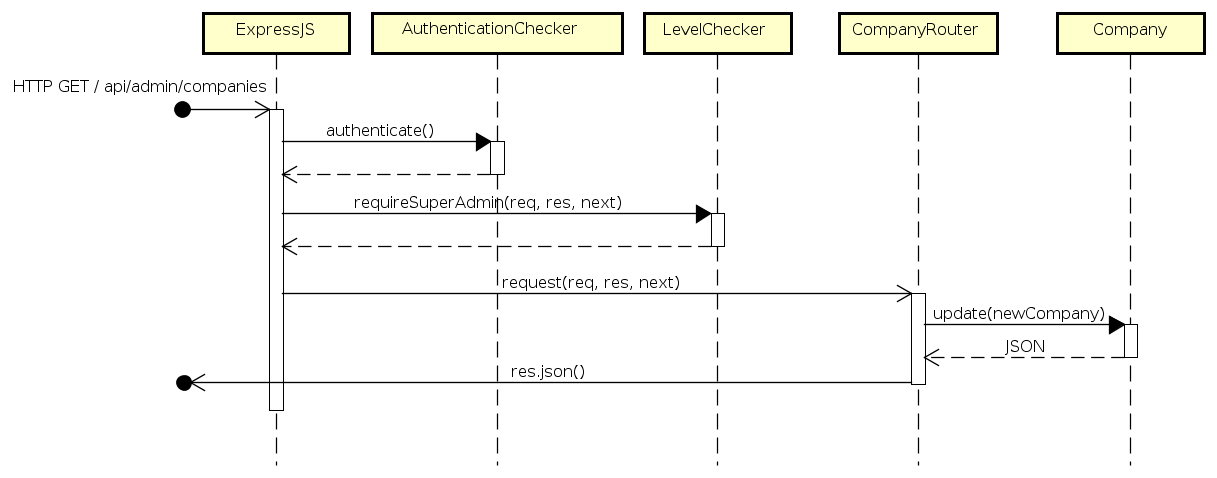
\includegraphics[width=0.8\textwidth]{res/sections/backend/sequence/(GET)companySA.png}
\caption{Scenario dell'ottenimento informazioni delle \glossaryItem{Company}}
\end{figure}

\newpage
\paragraph{Aggiunta di un SuperAdmin}\mbox{}\\
\textbf{Tipologia:} POST \\
\textbf{API:} /api/admin/superadmins \\
\textbf{Descrizione:} Necessita di una richiesta con \textit{body} contenente le informazioni relative al superadmin da creare, in particolare indirizzo email e password. L'indirizzo email deve essere unico: nel caso in cui questo vincolo non venga rispettato viene restituito un messaggio di errore; altrimenti viene ritornata una conferma di inserimento. \\
\textbf{Scenario:} 
\begin{figure}[H]
\centering
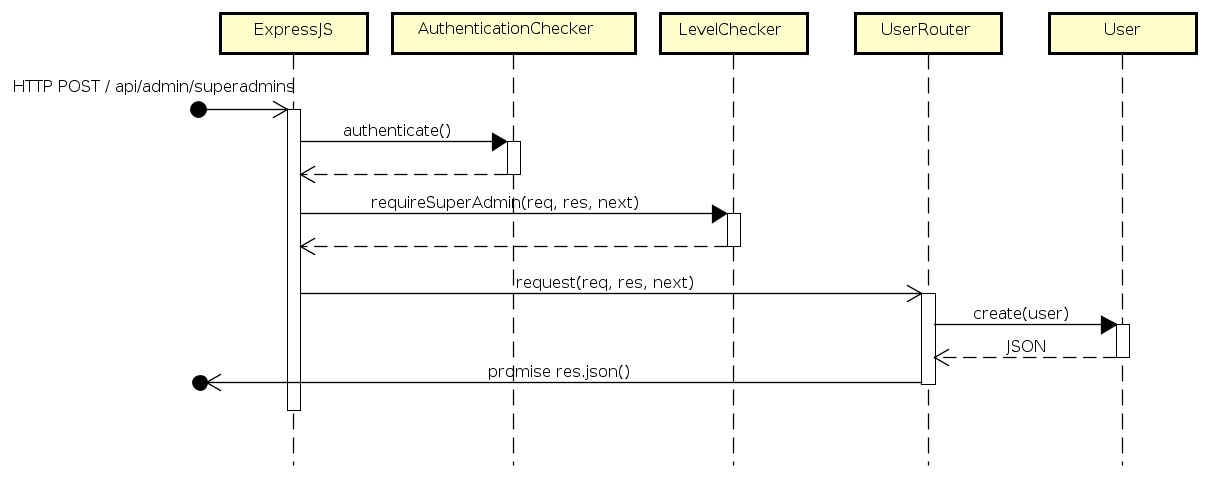
\includegraphics[width=0.8\textwidth]{res/sections/backend/sequence/(POST)superadmin.png}
\caption{Scenario dell'aggiunta di un super admin}
\end{figure}

\newpage
\paragraph{Aggiunta di un utente}\mbox{}\\
\textbf{Tipologia:} POST \\
\textbf{API:} /api/admin/companies/:company\_id/users \\
\textbf{Descrizione:} Necessita di una richiesta con \textit{body} contenente l'indirizzo email e il ruolo dell'utente da creare, che verrà associato alla \glossaryItem{Company} individuata da company\_id. \\
\textbf{Scenario:} 
\begin{figure}[H]
\centering
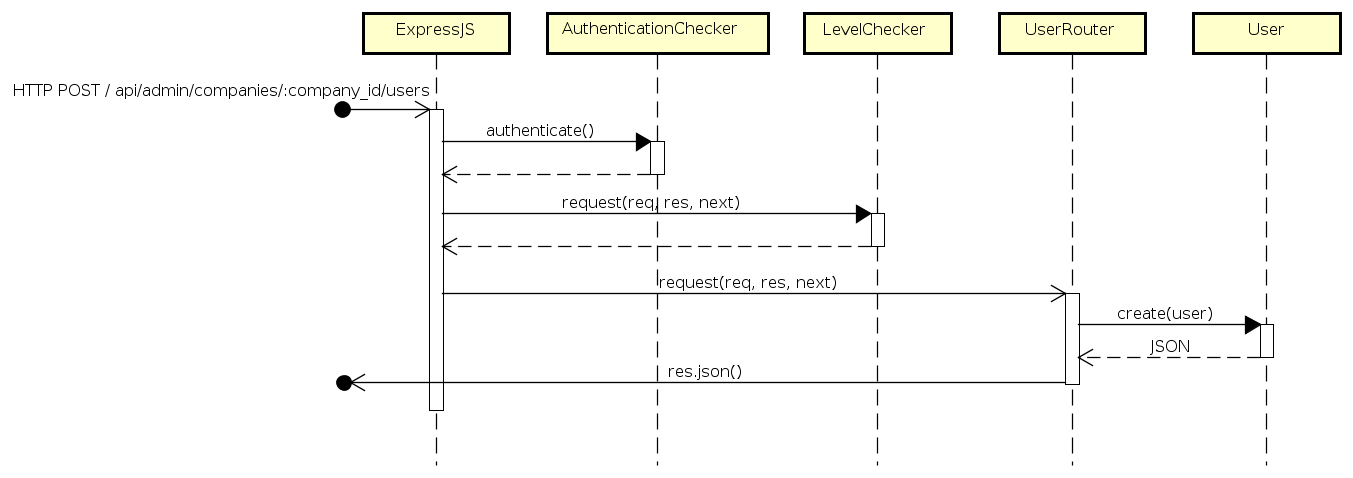
\includegraphics[width=0.8\textwidth]{res/sections/backend/sequence/(POST)userSA.png}
\caption{Scenario dell'aggiunta di un utente}
\end{figure}
